

\documentclass{cctbook}



% add package
 \usepackage{tocloft}
 \usepackage{graphicx}
 \usepackage{url}
 \usepackage{amsmath, amssymb}

\usepackage[colorlinks,linkcolor=blue,citecolor=blue,urlcolor=blue]{hyperref}
%\usepackage[colorlinks,linkcolor=black,citecolor=black,urlcolor=blue]{hyperref}
\usepackage[perpage]{footmisc} % The number of footnote will be reset on every new page.
\usepackage{eqlist}

% define new command
% ----------------------
% define
 \textheight 21.6cm
 \textwidth 14.5cm
 \topmargin  0pt
 \oddsidemargin=1.0cm
 \evensidemargin=1.0cm

 \pagestyle{plain}

%%%%%%%%%%%%%%%%%%%%%%%%%%%%%%%%%%%%
\makeatletter
\long\def\@makecaption#1#2{%
 \vskip\abovecaptionskip
 \sbox\@tempboxa{#2}%
 \ifdim \wd\@tempboxa >\hsize
   #2\par
 \else
   \global \@minipagefalse
   \hb@xt@\hsize{\hfil\box\@tempboxa\hfil}%
 \fi
 \vskip\belowcaptionskip}
\makeatother


% ----------------------
% define Content:
\renewcommand{\contentsname}{Abstracts}
 \renewcommand{\cftpartpresnum}{\quad}%{\quad  Part \ }
 \renewcommand{\cftpartaftersnum}{:}
\renewcommand\partname{Part \Roman{part}}
\newcommand{\Real}{\mathbb{R}}

 \cftbeforesecskip=4mm
% \renewcommand{\cftsecfont}{\parbox{11cm} }
\renewcommand{\cftsecfont}{\flushleft\vskip-7mm}
 \newcommand{\tcont}[2]{\addcontentsline{toc}{section}{{\bf #1}\\#2} \clearpage\phantomsection}

 \setcounter{tocdepth}{2}
% \clearemptypage

% ----------------------
% define general new command:
\newcommand{\bb}{\bigbreak}
\newcommand{\mb}{\medbreak}
\newcommand{\bc} {\begin{center}}
\newcommand{\ec}{\end{center}}
\newcommand{\np}{\newpage}
\newcommand{\und}[1]{\underline {\it #1 }}

% ----------------------
% commands needed by some paper
\def\Hnew{H_{\mbox{\scriptsize new}}}
\def\Hold{H_{\mbox{\scriptsize old}}}
\def\Wnew{H_{\mbox{\scriptsize new}}^{-1}}
\def\Wold{H_{\mbox{\scriptsize old}}^{-1}}

\def \fh{\dotfill \hbox{} \\ \hbox{}}
\newcommand{\lst}[2]{\par\vskip1mm \noindent \parbox[t]{6cm}{\small \bf #1:}
 \hskip5mm
\parbox[t]{8cm}{\small #2
}\vskip3mm}
\renewcommand\arraystretch{1.3}

\newcommand{\subj}[1]{{\Large\bf #1}}
\newcommand{\name}[1]{{\bf #1}\\[1mm]}
\newcommand{\dpt}[1]{#1\\}
\newcommand{\univ}[1]{#1\\}
\newcommand{\city}[1]{#1\\}
\newcommand{\email}[1]{Email: \href{mailto:#1}{\tt #1}\\[2mm]}


%---------------------------------------------------------------
%begin document
\begin{document}
%%%%%%%%%%%%%%%%%%%%%%%%%%%%%%%%%%%%%%%%%%%%%%%%%%%%%%%%%%%%%%%%%%%%%%%%%%
\frontmatter

\thispagestyle{empty} \vspace*{2cm}
\begin{center}
\LARGE\bf The 5th Sino-Japan Optimization Meeting \vskip12mm
\LARGE\sc September 26-29, 2011 \vskip6mm \LARGE Beijing, China
\vskip6mm
\LARGE\rm\texttt{http://lsec.cc.ac.cn/{\raise-.35ex\hbox{\textasciitilde}}sjom}
\end{center}

\begin{figure}
    \begin{center}
        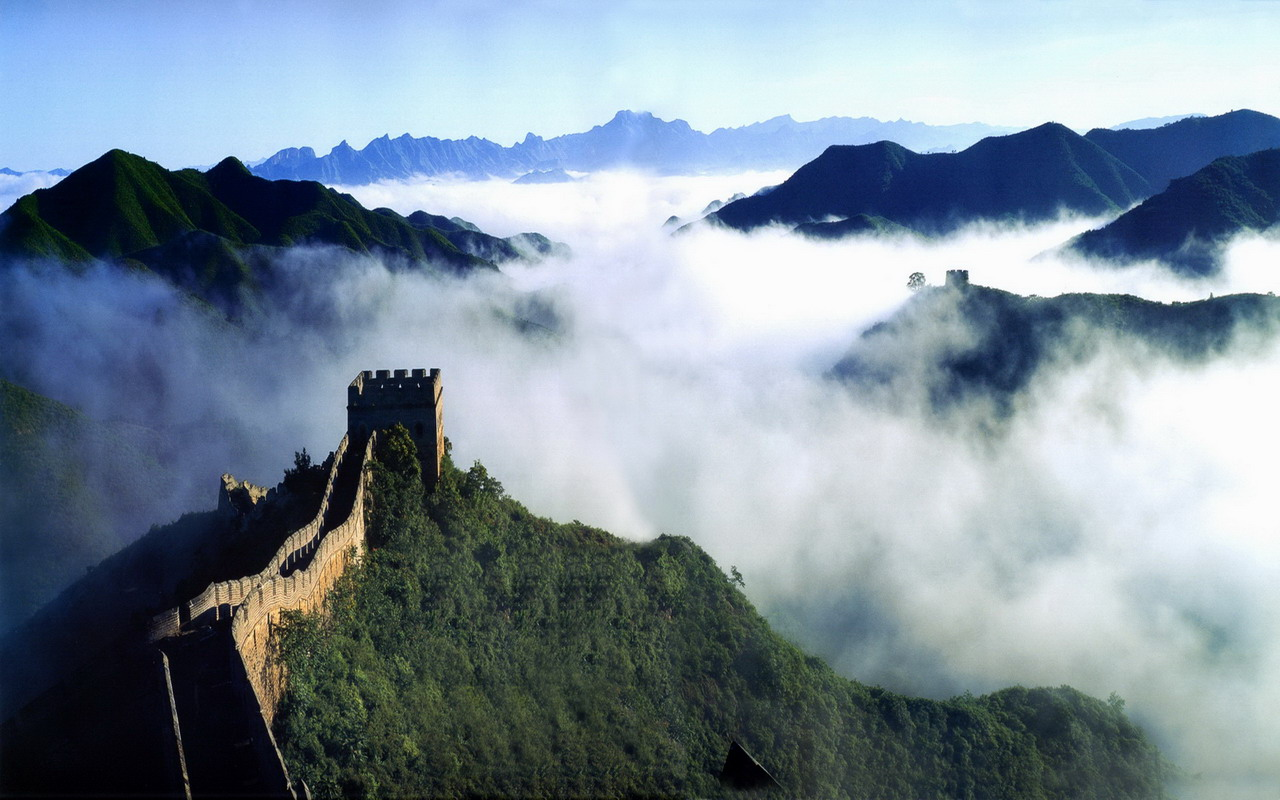
\includegraphics[width=1.0\textwidth]{GreatWall.jpg}
    \end{center}
\end{figure}


%%%%%%%%%%%%%%%%%%%%%%%%%%%%%%%%%%%%%%%%%%%%%%%%%%%%%%%%%%%%%%%%%%%%%%%%%%%%%%%%%%
% front pages
%\frontmatter
\newpage
\thispagestyle{empty}~~
%\newpage


\thispagestyle{empty}
\vspace*{2cm}
\begin{center}
\LARGE\bf The 5th Sino-Japan Optimization Meeting \vskip15mm
\LARGE\sc September 26-29, 2011 \vskip5mm \LARGE Beijing, China
\vskip5mm
 \LARGE\rm{\url{http://lsec.cc.ac.cn/~sjom }}
\vskip5mm
\LARGE\bf
---------------------------------------------------------\vskip5mm
 \hyperlink{INFO}{Information for Participants}\vskip2mm
 \hyperlink{SPON}{Sponsors}\vskip2mm
 \hyperlink{COM}{Committees} \vskip2mm
% \hyperlink{PROG}{Conference Program}\vskip2mm
 \hyperlink{SCH}{Conference Schedule} \vskip2mm
 \hyperlink{ABS}{Abstracts} \vskip2mm
 \hyperlink{LST}{List of Participants}\vskip2mm
 \hyperlink{SIGHT}{Sightseeing Information}
\end{center}

%%%%%%%%%%%%%%%%%%%%%%%%%%%%%%%%%%%%%%%%%%%%%%%%%%%%%%%%%%%%%%%%%%%%%%%%%%%%%%%%
%\let\flag\true
%\ifx\flag\true \else fi

%\newpage
\thispagestyle{empty}~~
\newpage
\setcounter{page}{1}
%\vspace*{10mm}
\begin{center}
\rm
%\thispagestyle{empty}
\hypertarget{INFO}{\normalsize {\LARGE \bf Information for
Participants}} \vskip12mm
\end{center}
\Large \rm

\begin{center}
{\bf Conference Site}\\~\vspace{-0.3cm}\\
 \hspace{-0.45cm}
\begin{tabular}{lp{0.7\textwidth}p{\textwidth}}
\centering
Conference Site:&Si-Yuan Building, Academy of Mathematics and Systems Science (AMSS), Chinese Academy of Sciences (CAS)\\
%Chinese Name:&\mbox{�п�Ժ��ѧ��ϵͳ��ѧ�о�Ժ˼Դ¥}\\
Address:&No. 55, Zhong Guan Cun East Road, Hai Dian District, Beijing, CHINA\\
%Chinese Address:&\mbox{�����к������йش嶫·\,55\,��}
\end{tabular}
\end{center}

%\bigskip
%\begin{center}
%\sf Arrival \& Departure
%\end{center}
%
%There will be volunteers waiting for you at the airport when you
%arrive, if you have sent your arrival information to the organizing
%committee. They will help you to call a taxi to our conference
%hotel.
%
%We will arrange volunteers to send you to the airport when you
%leave, if you have sent your departure information to the organizing
%committee.
\bigskip

\begin{center}
\bf Reception \& On-site Registration
\end{center}

Reception and on-site registration will take place simultaneously in
two venues on September 25:
\begin{eqlist}
  \item[~~~~~~~$\bullet$] September 25, 9:00-18:00, lobby of Jade Palace Hotel.
  \item[~~~~~~~$\bullet$] September 25, 9:00-18:00, lobby of Institute of Computational Mathematics and Scientific/Engineering Computing (ICMSEC), AMSS, CAS.
\end{eqlist}

If you are accommodated at Jade Palace, please register at the
hotel; otherwise, please register at ICMSEC, AMSS, CAS. If you want
to register at other time, please contact our conference secretary
\href{mailto:wjp@lsec.cc.ac.cn}{Ms. Ji-ping Wu}.
\bigskip

\begin{center}
\bf Currency
\end{center}

Chinese currency is RMB. The current rate is about 6.38 RMB for 1 US
dollar. The exchange of foreign currency can be done at the airport
or the conference hotel (Jade Palace Hotel). Please keep the receipt
of the exchange so that you can change back to your own currency if
you have RMB left before you leave China.


\bigskip
\begin{center}
\bf From Jade Palace to AMSS
\end{center}

For participants accommodated at Jade Palace: in each morning of
September 26-28, Dr. Xin Liu and Miss Cong Sun will guide you to the
conference site at AMSS. You will set off punctually at 8:00 a.m.,
from the lobby of Jade Palace. Please wait in the lobby in advance.
There will be only one guidance each morning. If you miss it, you
will have to go to the conference site by yourself.

\bigskip
\begin{center}
\bf Contact Information
\end{center}

If you need any help, please contact the conference secretaries:
\begin{eqlist}
 \item[~~~~~~~$\bullet$] \href{mailto:wjp@lsec.cc.ac.cn}{Ms. Ji-ping Wu}: +86-136-9106-6084~(in
 Chinese).
 \item[~~~~~~~$\bullet$] \href{mailto:zhangzk@lsec.cc.ac.cn}{Mr. Zaikun Zhang}:
 +86-159-0152-1357.
\end{eqlist}


\begin{figure}
\caption{\Large \bf Local Map}
    \begin{center}
        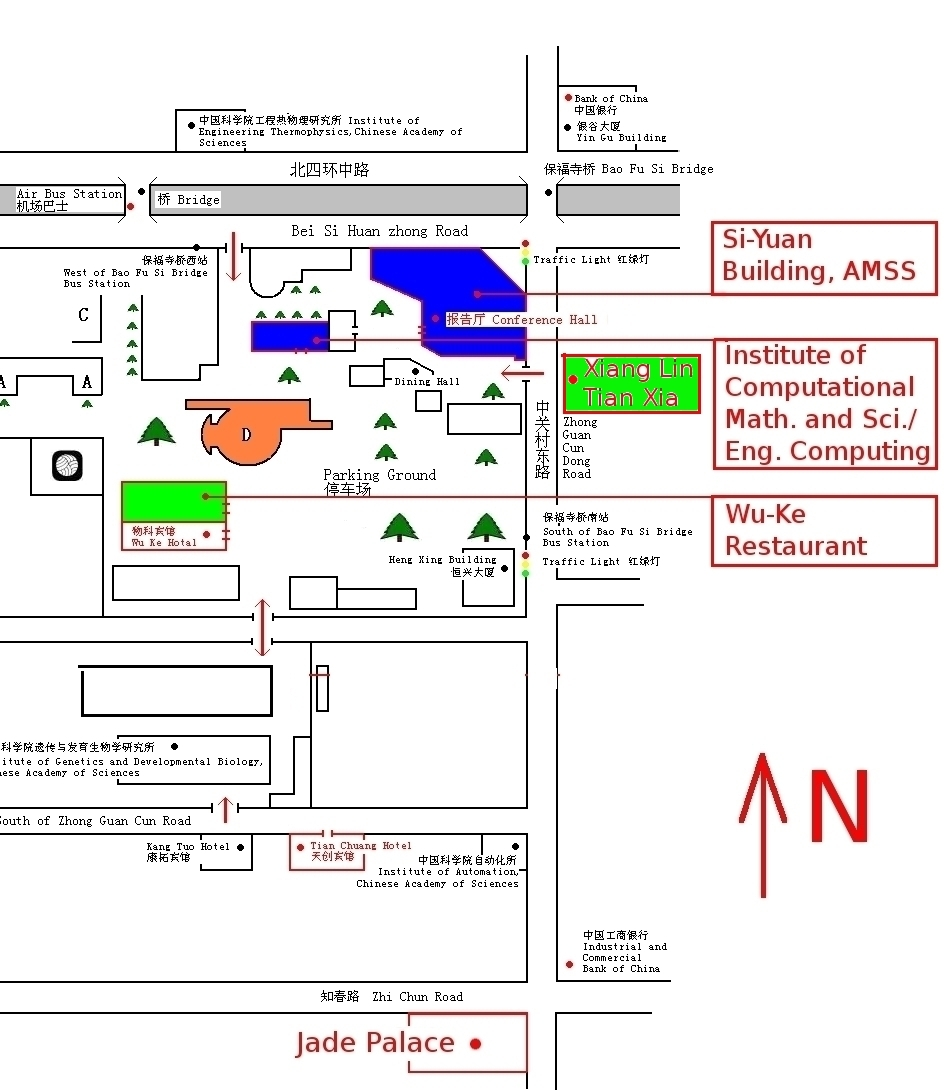
\includegraphics[width=1.0\textwidth]{localmap.jpg}
    \end{center}
\end{figure}

%%%%%%%%%%%%%%%%%%%%%%%%%%%%%%%%%%%%%%%%%%%%%%%%%%%%%%%%%%%%%%%%%%%%%%%%%%%%%%%
\newpage

\begin{center}
\rm
%\thispagestyle{empty}
\hypertarget{SPON}{\normalsize {\LARGE \bf Sponsors}} \vskip12mm
\end{center}

\begin{center}
 \rm
National Natural Science Foundation of China \\[5mm]

Chinese Academy of Sciences \\[5mm]

Academy of Mathematics and Systems Science\\[5mm]

State Key Laboratory of Scientific and Engineering Computing\\[5mm]

Institute of Computational Mathematics and Scientific/Engineering
Computing\\[5mm]

Center for Optimization and Applications, AMSS
\end{center}
%%%%%%%%%%%%%%%%%%%%%%%%%%%%%%%%%%%%%%%%%%%%%%%%%%%%%%%%%%%%%%%%%%%%%%%%%%%%%%%%


\newpage

\begin{center}
\rm
%\thispagestyle{empty}
\hypertarget{COM}{\normalsize {\LARGE \bf Committees}} \vskip12mm
\end{center}

\begin{center}
 \rm
 {\Large \bf Steering Committee} \\[10mm]

X.J. Chen (Hong Kong Polytechnic University)\\[5mm]

S. Fujishige (Kyoto University)\\[5mm]

M. Fukushima (Kyoto University)\\[5mm]

J.Y. Han (Chinese Academy of Sciences)\\[5mm]

B.S. He (Nanjing University)\\[5mm]

H. Kawasaki (Kyushu University)\\[5mm]

M. Kojima (Tokyo Institute of Technology)\\[5mm]

M. Kubo (Tokyo University of Marine Science and Technology)\\[5mm]

D. Li (Chinese University of Hong Kong)\\[5mm]

L.Z. Liao (Hong Kong Baptist University)\\[5mm]

S. Mizuno (Tokyo Institute of Technology)\\[5mm]

K. Murota (University of Tokyo)\\[5mm]

H. Nagamochi (Kyoto University)\\[5mm]

L.Q. Qi (Hong Kong Polytechnic University)\\[5mm]

J. Sun (National University of Singapore)\\[5mm]

W.Y. Sun (Nanjing Normal University) ({\bf Co-Chair})\\[5mm]

X.L. Sun (Fudan University)\\[5mm]

A. Tamura (Keio University)\\[5mm]

T. Tanaka (Niigata University)\\[5mm]

T. Tanino (Osaka University) ({\bf Co-Chair})\\[5mm]

K.L. Teo (Curtin University) \\[5mm]

T. Tsuchiya (National Graduate Institute for Policy Studies) \\[5mm]

S.Y. Wang (Chinese Academy of Sciences) \\[5mm]

S.Y. Wu (National Cheng Kung University) \\[5mm]

H. Yabe (Tokyo University of Science) \\[5mm]

H. Yamashita (Mathematical Systems, Inc.) \\[5mm]

X.M. Yang (Chongqin Normal University) \\[5mm]

A. Yoshise (University of Tsukuba) \\[5mm]

Y.X. Yuan (Chinese Academy of Sciences) \\[5mm]

J.Z. Zhang (City University of Hong Kong) \\[5mm]

X.S. Zhang (Chinese Academy of Sciences) \\[15mm]


{\Large \bf Organizing Committee} \\[10mm]

Yu-Hong Dai (Chinese Academy of Sciences, China) \\[5mm]

Masao Fukushima (Kyoto Univeristy, Japan) \\[5mm]

Xin Liu (Chinese Academy of Sciences, China) \\[5mm]

Wenyu Sun (Nanjing Normal University, China) \\[5mm]

Naihua Xiu (Beijing Jiaotong University, China) \\[5mm]

Ya-Xiang Yuan (Chinese Academy of Sciences) ({\bf Chair})

\end{center}


%%%%%%%%%%%%%%%%%%%%%%%%%%%%%%%%%%%%%%%%%%%%%%%%%%%%%%%%%%%%%%%%%%%%%%%%%%%%%%%%%
%
%\newpage
%\begin{center}
%\rm %\thispagestyle{empty}
%\hypertarget{PROG}{\normalsize {\LARGE \bf Conference Program}}
%\vskip12mm
%\end{center}
%\LARGE \rm
%\begin{itemize}
%\item September 25, Reception and On-site Registration
%\item September 26-28, Plenary and Contributed Talks
%%\begin{itemize}
%%\item {\Large Check \hyperlink{SCH}{\bf Conference Schedule} for details.}
%%\end{itemize}
%\item September 29, Sightseeing
%%\begin{itemize}
%%\item {\Large Morning, Great Wall.}
%%\item {\Large Afternoon, Ming Dynasty Tombs.}
%%\end{itemize}
%\end{itemize}
%

%%%%%%%%%%%%%%%%%%%%%%%%%%%%%%%%%%%%%%%%%%%%%%%%%%%%%%%%%%%%%%%%%%%%%%%%%%%%%%%
\newpage
\normalsize

\begin{center}
\rm \hypertarget{SCH}{\normalsize {\LARGE \bf The 5th Sino-Japan
Optimization Meeting\\[3mm]{\sc September 26-29, 2011}\\[3mm]{\sc Beijing, China}\\[7mm]Conference Schedule}} \vskip12mm
\end{center}
%
%
\newcommand{\whday}[1]{\begin{flushleft}
{\Large \bf \underline{#1}}
\end{flushleft}}

\newcommand{\where}[1]{{(\bf#1)}}
\newcommand{\chair}[1]{{\bf Chair:~#1}}
%\newcommand{\chair}{Chair:~~~~~~~~~~~}
\newenvironment{schedule}{\begin{eqlist}\large}{\end{eqlist}}
\newenvironment{talks}{\begin{eqlist}\normalsize}{\end{eqlist}}
\newcommand{\sitem}[2]{\item[\bf#1~]{\bf#2}}
\newcommand{\talk}[3]{\item[\bf#1~]{\bf#2},~#3}

\newcommand{\LHSY}{Lecture Hall, Si-Yuan
Building}
\newcommand{\SSY}{Room 712, Si-Yuan
Building}


\whday{September 26, Monday}

\setlength{\itemsep}{10mm}

\begin{schedule}
\sitem{08:30-09:10}{Opening Ceremony \\\where{Lecture Hall, Si-Yuan
Building}}
\begin{talks}
\sitem{08:30-08:50}{Welcome Address}

\sitem{08:50-09:10}{Group Photo}
\end{talks}

\sitem{09:10-09:30}{Coffee Break}

\sitem{09:30-12:00}{Invited Talks I1 \\\chair{Wenyu Sun}
\where{\LHSY}}
\begin{talks}
\talk{09:30-10:20}{Tam\'{a}s Terlaky}{Cone Linear Optimization
(CLO): from LO, SOCO and SDO towards mixed integer CLO}

\talk{10:20-11:10}{Mikio Kubo}{Trend in Supply Chain Optimization
and Humanitarian Logistics }

\talk {11:10-12:00} {Xiaoling Sun} {Modeling and Algorithmic
Challenges from Financial Optimization}
\end{talks}

\sitem{12:00-13:30}{Lunch \where{4th Floor, Wu-Ke Restaurant}}

\sitem{13:30-15:10}{Invited Talks I2 \\\chair{Tetsuzo Tanino}
\where{\LHSY}}

\begin{talks}
\talk {13:30-14:20}{Soon-Yi Wu}{On finite convergence of an explicit
exchange method for convex semi-definite programming problems with
second-order cone constraints}

\talk{14:20-15:10}   {Zaiwen Wen} {Optimization with orthogonality
constraints and its applications}

\end{talks}

\sitem{15:10-15:30} {Coffee Break}

\sitem{15:30-18:30}{ Contributed Talks C1 \& C2}

\sitem{\phantom{15:30-18:30}}{C1, \chair{Mikio Kubo} \where{\LHSY}}

\begin{talks}
\talk{15:30-16:00}   {Shinji Mizuno} {Klee-Minty's LP and Upper
Bounds for Dantzig's Simplex Method}

\talk{16:00-16:30}   {\underline{Xin Liu}} {Limited Memory Block
Krylov Subspace Optimization for Computing Dominant Singular Value
Decompositions (\bf{Changed})}

\talk {16:30-17:00}   {Chao Zhang} {A New Active Set Method For
Nonnegative Matrix Factorization}

\talk{17:00-17:30}   {Jiming Peng}{Sparse Solutions to Classes of
Quadratic Programming Problems }

\talk{17:30-18:00}  {Wei Bian} {Smoothing Neural Network for
Constrained Non-Lipschitz Optimization with Applications}

\talk{18:00-18:30}   {Yanfang Zhang} {Moreau-Yosida regularization
for stochastic linear variational inequalities}
\end{talks}

\sitem{\phantom{15:30-18:80}}{C2, \chair{Yu-Hong Dai} \where{\SSY}}

\begin{talks}
\talk{15:30-16:00}   {\underline{Rui Diao}} {A  New Family of Matrix
Completion Quasi-Newton Methods ({\bf Changed})}

\talk{ 16:00-16:30}   {Mituhiro Fukuda} {High performance software
package for SDP: SDPA version 7}

\talk{ 16:30-17:00} {Wanyou Cheng} {An Adaptive Gradient Algorithm
for Large-scale Nonlinear Bound Constrained Optimization}

\talk{17:00-17:30} {\underline{Cong Sun}} {A Hybrid Algorithm for
Power Maximization Interference Alignment Problem of MIMO Channels}

\talk{17:30-18:00}   {Zaikun Zhang} {Sobolev Seminorm of Quadratic
Functions with Applications to Derivative-Free Optimization}


\talk{18:00-18:30} {Zhengyong Zhou} {A discretization method for
nonlinear semi-infinite programming based on the flatten aggregate
constraint homotopy method for solving the discretized problem}
\end{talks}

%\sitem{\mbox{}\phantom{18:40-}18:40} {Dinner \where{Xiang Lin Tian
%Xia Restaurant}}

\sitem{18:40} {Dinner \where{Xiang Lin Tian Xia Restaurant}}

\sitem{20:00} {SJOM Steering Committee Meeting \\\where{Room 305,
Institute of Computational Mathematics and Scientific/Engineering
Computing}}

\end{schedule}

\np

\whday{September 27, Tuesday}

\begin{schedule}

\sitem{08:30-10:10} {Invited Talks I3\\\chair{Masao Fukushima}
\where{\LHSY} }
\begin{talks}
\talk{08:30-09:20}   {Xiaojun Chen} {Expected Residual Minimization
for Stochastic Variational Inequalities}

\talk{ 09:20-10:10}  {Marc Teboulle} {First Order Algorithms for
Well Structured Optimization Problems}
\end{talks}

\sitem{10:10-10:30} {Coffee Break}

\sitem{10:30-12:00} {Contributed Talks C3 \& C4}

\sitem{\phantom{10:000-10:00}}{C3, \chair{Xiaojun Chen}
\where{\LHSY}}
\begin{talks}
\talk{10:30-11:00}   {Bingsheng He} {on the $O(1/t)$ convergence
rate of the alternating direction methods for convex optimization
and monotone variational inequalities}

\talk{11:00-11:30}  {Keiji Tatsumi} {A sufficient condition for
chaos in a steepest decent system with sinusoidal perturbation for
global optimization}

\talk{ 11:30-12:00}  {Bo Jiang} {An improved model for truck
dispatching in open pit mine}
\end{talks}

\sitem{\phantom{10:000-10:00}}{C4, \chair{Satoru Iwata}
\where{\SSY}}

\begin{talks}
\talk{10:30-11:00}  {Shunsuke Hayashi} {Semi-infinite program with
infinitely many conic constraints: optimality condition and
algorithms}

\talk{ 11:00-11:30}   {Ryan Loxton} {Optimal Control Problems with
Stopping Constraints}

\talk{ 11:30-12:00}   {Lishun Zeng} {On the Separation in 2-Period
Double Round Robin Tournaments with Minimum Breaks}
\end{talks}

\sitem{12:00-13:30} {Lunch \where{4th Floor, Wu-Ke Restaurant}}

\sitem{13:30-15:10} {Invited Talks I4 \\\chair{Naihua Xiu}
\where{\LHSY}}
\begin{talks}
\talk{13:30-14:20}   {Hiroshi Yamashita} {Primal-dual Interior Point
Methods for Nonlinear SDP  - Local and Global Analysis}

\talk{14:20-15:10} {Yu-Hong Dai} {Joint Power and Admission Control
for a SISO Interference Channel: Complexity Analysis, Algorithm
Design, and Distributed Implementation}
\end{talks}
\sitem{15:10-15:30} {Coffee Break}

\sitem{15:30-17:00} {Contributed Talks C5 \& C6}

\sitem{\phantom{00:00-00:00}}{C5, \chair{Hiroshi Yamashita}
\where{\LHSY}}
\begin{talks}
\talk{15:30-16:00}   {Naihua Xiu} {$S$-goodness: Low-Rank Matrix
Recovery from Sparse Signal Recovery}

\talk{ 16:00-16:30}   {Hidefumi Kawasaki} {An application of a
discrete fixed point theorem for contraction mappings to a game in
expansive form}

\talk{ 16:30-17:00} {Lingchen Kong} {Exact Low-rank Matrix Recovery
via Nonconvex $M_p$-Minimization}
\end{talks}

\sitem{\phantom{00:00-00:00}}{C6, \chair{Jiawang Nie} \where{\SSY}}

\begin{talks}
\talk{15:30-16:00}   {Qun Lin} {Optimal Fleet Sizing via Dynamic
Programming and Golden Section Search}

\talk{16:00-16:30}   {Yasushi Narushima} {A smoothing conjugate
gradient method for solving nonsmooth systems of equations}

\talk{16:30-17:00}  {Lei Guo} {M-Stationarity and Stability Analysis
for Mathematical Programs with Complementarity Constraints}
\end{talks}
%\sitem{\mbox{}\phantom{00:00-}17:10} {Bus to Conference Banquet\\
%\where{Conference Banquet at Summer Palace}}
\sitem{17:10}{Dinner \where{3rd Floor, Wu-Ke Restaurant}}
\end{schedule}

\np

\whday{September 28, Wednesday}

\begin{schedule}

\sitem{08:30-10:10} {Invited Talks I5 \\\chair{Jie Sun}
\where{\LHSY}}
\begin{talks}
\talk{08:30-09:20}   {Yin Zhang} {Some Recent Advances in
Alternating Direction Methods: Practice and Theory}

\talk{ 09:20-10:10}   {Satoru Iwata} {Submodular Optimization and
Approximation Algorithms}
\end{talks}

\sitem{10:10-10:30} {Coffee Break}

\sitem{10:30-12:00} {Contributed Talks C7 \& C8}

\sitem{\phantom{00:00-00:00}}{C7, \chair{Bingsheng He}
\where{\LHSY}}
\begin{talks}
\talk{10:30-11:00}   {Hiroshi Yabe} {Conjugate gradient methods
based on secant conditions that generate descent search directions
for unconstrained optimization}

\talk{ 11:00-11:30}   {Xiao Wang} {An Augmented Lagrangian Trust
Region Algorithm for Equality Constrained Optimization}

\talk{ 11:30-12:00} {Congpei An} {Regularized least squares
approximation over the unit sphere using spherical designs}
\end{talks}
\sitem{\phantom{00:00-00:00}}{C8, \chair{Zaiwen Wen} \where{\SSY}}

\begin{talks}
\talk{10:30-11:00}   {Ying Lu} {Plan Postponement Strategy: A
Definition and Research Model}

\talk{ 11:00-11:30}   {Min Li} {Inexact Solution of NLP Subproblems
in MINLP}

\talk{ 11:30-12:00}   {Atsushi Kato} {Global and superlinear
convergence of inexact sequential quadratically constrained
quadratic programming method for convex programming}
\end{talks}

\sitem{12:00-13:30} {Lunch \where{4th Floor, Wu-Ke Restaurant}}

\sitem{13:30-15:10} {Invited Talks I6\\\chair{Soon-Yi
Wu}\where{\LHSY}}

\begin{talks}
\talk{13:30-14:20}   {Lu\'{i}s Nunes  Vicente} {Sparse and Smoothing
Methods for Nonlinear Optimization Without Derivatives}

\talk{ 14:20-15:10} {Ye Lu} {Optimal Policy for an Inventory System
with Convex Variable Cost and a Fixed Cost}
\end{talks}

\sitem{15:10-15:30} {Coffee Break}


\sitem{15:30-16:20} {Invited Talks I7\\\chair{Yin Zhang}
\where{\LHSY}}

\begin{talks}
\talk{15:30-16:20}   {Jiawang Nie} {Jacobian SDP Relaxation for
Polynomial Optimization}
\end{talks}

\sitem{16:20-16:30} {Closing Ceremony\\\where{\LHSY}}

%\sitem{\mbox{}\phantom{00:00-}17:30} {Dinner \where{3rd Floor, Wu-Ke
%Restaurant}}
\sitem{16:50} {Bus to Conference Banquet\\
\where{Conference Banquet at Da Zhai Men Restaurant}}

\end{schedule}

\np

\whday{September 29, Thursday}
\begin{schedule}
\sitem{7:00} {Set off from Jade Palace}

\sitem{Morning} {Half-day Tour to Great Wall}

\sitem{Afternoon}{Half-day Tour to Ming Dynasty Tombs}

%\sitem{Dinner}{Hot Pot}
\end{schedule}

%add contents
 \clearpage
 \hypertarget{ABS}{}\tableofcontents
 \clearpage


%begin abstract
\mainmatter


%Invited talks
\part{Invited Talks}
%\clearpage

%--------------------------------------------------------------1
%--------------------------------------------------------------1

\bc \subj{Expected Residual Minimization for Stochastic Variational
Inequalities}\bb\name{Xiaojun Chen}\dpt{Department of Applied
Mathematics}\univ{The Hong Kong Polytechnic University}\city{Hong
Kong}\email{maxjchen@polyu.edu.hk} \ec\bb\bb

The stochastic variational inequality (SVI) has been used widely in
engineering and economics, as an effective mathematical model for a
number of equilibrium problems involving uncertain data.  We present
an expected residual minimization (ERM) formulation for a class of
SVI, including the complementarity problem as a special case. The
objective of the ERM-formulation is Lipschitz continuous and
semismooth which helps us guarantee the existence of a solution and
convergence of approximation methods. Moreover, this minimization
problem is convex for linear SVI if the expected matrix is positive
semi-definite. We propose a globally convergent (a.s.) smoothing
sample average approximation (SSAA) method
 to minimize the residual function.  We show that the ERM problem and its SSAA problems
have minimizers in a compact set and any cluster point of minimizers
and stationary points of the SSAA problems is a minimizer and a
stationary point of the ERM problem (a.s.).  We illustrate the ERM
and SSAA by examples from traffic equilibrium assignment problems.

\tcont{Expected Residual Minimization for Stochastic Variational
Inequalities}{Xiaojun Chen}

\np

%--------------------------------------------------------------2
%--------------------------------------------------------------2

\bc \subj{Joint Power and Admission Control for a SISO Interference
Channel: Complexity Analysis, Algorithm Design, and Distributed
Implementation}\bb\name{Yu-Hong Dai}\dpt{Institute of Computational
Mathemtaics and Scientific/Engineering Computing} \univ{Chinese
Academy of Sciences} \city{Beijing 100190,
China}\email{dyh@lsec.cc.ac.cn} \ec\bb\bb

Power control, aiming at providing each user in the interference
channel with the prescribed quality of service (QoS) target, has
been extensively studied. However, when there are too many
co-channel users, it is not possible to simultaneously satisfy all
users' QoS requirements due to mutual interferences and individual
power limits. Therefore, it is necessary to bring up the admission
control, and makes sense to maximize the number of admitted users at
their desired QoS demands. It is shown that the joint power and
admission control problem is strongly NP-hard and there even does
not exist a polynomial-time approximation algorithm for it; hence,
convex approximation heuristics approaches are considered. We first
reformulate the problem as a sparse $\ell_0$-minimization problem
and then relax it to a linear programming. Next, two easy-checking
necessary conditions that all users in the network can be
simultaneously supported are derived. Based on above analysis, a new
linear programming deflation (NLPD) algorithm is proposed, which
minimizes a weighted summation of the total excess transmission
power and the total real transmission power in each step. The
distributed implementation of NLPD is also developed since the
network often suffers a large communication overhead for the
implementation of a centralized algorithm. The projected alternate
Barzilai-Borwein (PABB) algorithm with the continuation technique is
proposed to carry out the power control. The proposed algorithm not
only allows each node to locally update its power with limited
information exchange, but also preserves the high computational
efficiency of the centralized algorithm. Numerical simulations show
the proposed centralized and distributed algorithms outperform
state-of-the-arts.

This work is jointed with Ya-feng Liu and Zhiquan Luo.


\tcont{Joint Power and Admission Control for a SISO Interference
Channel: Complexity Analysis, Algorithm Design, and Distributed
Implementation}{Yu-Hong Dai}

\np

%--------------------------------------------------------------3
%--------------------------------------------------------------3

\bc \subj{Submodular Optimization and Approximation
Algorithms}\bb\name{Satoru Iwata}\dpt{Research Institute for
Mathematical Sciences (RIMS)}\univ{Kyoto University}\city{Kyoto
606-8502, Japan}\email{iwata@kurims.kyoto-u.ac.jp} \ec\bb\bb

Submodular functions are discrete analogues of convex functions.
Examples include cut capacity functions, matroid rank functions, and
entropy functions. Submodular functions can be minimized in
polynomial time, which provides a fairly general framework of
efficiently solvable combinatorial optimization problems. In
contrast, the maximization problems are NP-hard and several
approximation algorithms have been developed so far.

In this talk, I will review the above results in submodular
optimization and present recent approximation algorithms for
combinatorial optimization problems described in terms of submodular
functions.

\tcont{Submodular Optimization and Approximation Algorithms}{Satoru
Iwata}

\np

%--------------------------------------------------------------4
%--------------------------------------------------------------4

\bc \subj{Trend in Supply Chain Optimization and Humanitarian
Logistics}\bb\name{Mikio Kubo}\dpt{Department of Information
Engineering and Logistics}\univ{Tokyo University of Marine Science
and Technology}\city{12-5 Echujima Koutou-ku, Tokyo 135-0083,
Japan}\email{kubo@kaiyodai.ac.jp} \ec\bb\bb

In this talk, we survey the supply chain (SC) optimization. We
introduce three decision levels of the SC, show the classification
of inventories, and then discuss several basic optimization models
such as logistics network design, inventory, scheduling, lot-sizing,
and vehicle routing models. We also review recent progress in
humanitarian logistics and supply chain risk management.

\tcont{Trend in Supply Chain Optimization and Humanitarian
Logistics}{Mikio Kubo}

\np

%--------------------------------------------------------------5
%--------------------------------------------------------------5

\bc \subj{Optimal Policy for an Inventory System with Convex
Variable Cost and a Fixed Cost}\bb\name{Ye Lu}\univ{City University
of Hong Kong}\city{Hong Kong}\email{yelu22@cityu.edu.hk} \ec\bb\bb

We study the optimal policy for a periodic-review inventory system
where there is a fixed cost and the variable ordering cost is
defined by a piece-wise linear convex  function. By introducing the
concept of strong (K,c,q)-convexity, we characterize the structure
of the optimal policy. Based on this structure, we propose a well
performed heuristics algorithm to solve this problem.

\tcont{Optimal Policy for an Inventory System with Convex Variable
Cost and a Fixed Cost }{Ye Lu}

\np

%--------------------------------------------------------------6
%--------------------------------------------------------------6

\bc \subj{Jacobian SDP Relaxation for Polynomial Optimization
}\bb\name{Jiawang Nie}\dpt{Mathematics Department}\univ{University
of California, San Diego (UCSD)}\city{9500 Gilman Drive, La Jolla,
CA 92093, USA}\email{njw@math.ucsd.edu} \ec\bb\bb

Consider the global optimization problem of minimizing a polynomial
function subject to polynomial equalities and/or inequalities.
Jacobian SDP Relaxation is the first method that can solve this
problem globally and exactly by using semidefinite programming. This
solves an open problem in the field of polynomial optimization. Its
basic idea is to use the minors of Jacobian matrix of the given
polynomials,  add new redundant polynomial equations about the
minors to the constraints,  and then apply the hierarchy of
Lasserre's semidefinite programming relaxations. The main result is
that this new semidefinite programming relaxation will be exact for
a sufficiently high (but finite) order, that is, the global minimum
of the polynomial optimization can be computed by solving a
semidefinite programming problem.

\tcont{Jacobian SDP Relaxation for Polynomial Optimization}{Jiawang
Nie}

\np

%--------------------------------------------------------------7
%--------------------------------------------------------------7

\bc \subj{Modeling and Algorithmic Challenges from Financial
Optimization}\bb\name{Xiaoling Sun}\dpt{School of
Management}\univ{Fudan University}\city{670 Guoshun Road, Shanghai
200433, China}\email{xls@fudan.edu.cn} \ec\bb\bb

In this talk, we discuss some modeling and algorithmic challenges
from financial optimization.

We consider portfolio selection models with three types of hard
constraints arising from real-world trading practice:
\\\indent(i) cardinality constraint;
\\\indent(ii) probabilistic constraints; \\\indent(iii) marginal risk constraints.

These portfolio selection models are of NP-hard optimization
problems. We propose some new reformulations and convex relaxation
techniques.

Preliminary numerical results will be also reported.

\tcont{ Modeling and Algorithmic Challenges from Financial
Optimization}{Xiaoling Sun}

\np

%--------------------------------------------------------------8
%--------------------------------------------------------------8

\bc \subj{First Order Algorithms for Well Structured Optimization
Problems}\bb\name{Marc Teboulle}\dpt{School of Mathematical
Sciences}\univ{Tel Aviv University }\city{Ramat Aviv, Tel Aviv
69978, Israel}\email{teboulle@post.tau.ac.il} \ec\bb\bb

Many fundamental scientific and engineering problems of recent
interest arising in signal recovery, image processing, compressive
sensing, machine learning and other fields can be formulated as well
structured optimization problems, but which are typically very large
scale, and often nonsmooth and nonconvex. This leads to challenging
difficulties for their solutions, precluding the use of most well
established sophisticated algorithms, such as interior point.
Elementary first order methods then often remain our best
alternative to tackle such problems.\medskip

This talk surveys recent results on the design and analysis of
gradient-based algorithms for some generic optimization models
arising in a wide variety of applications, highlighting the ways in
which problem structures can be beneficially exploited to devise
simple and efficient algorithms.

\tcont{First Order Algorithms for Well Structured Optimization
Problems}{Marc Teboulle}

\np

%--------------------------------------------------------------9
%--------------------------------------------------------------9

\bc \subj{Cone Linear Optimization (CLO): \\{\large from LO, SOCO
and SDO towards  mixed integer CLO} }\bb\name{Tam\'{a}s
Terlaky}\dpt{ Harold S. Mohler Laboratory}\univ{Lehigh
University}\city{200 West Packer Avenue, Bethlehem, PA 18015-1582,
USA}\email{terlaky@lehigh.edu} \ec\bb\bb

Cone Linear Optimization (CLO) has been the subject of intense study
in the past two decades. Interior Point Methods (IPMs) provide
polynomial time algorithms in theory, and powerful software tools in
computational practice. The applications of Second-Order Conic
(SOCO) and Semi-Definite Optimization (SDO) expanded rapidly. The
first part of this talk reviews model formulation, IPM fundamentals,
available software and some applications of CLO problems.

The use of integer variables naturally occur in CLO problems too,
thus the need for dedicated mixed integer CLO algorithms and
software is evident. The second part of this talk gives some insight
of how to design disjunctive conic cuts for mixed integer CLO
problems.

\bb\bb

{\flushleft\large{\bf Biography:}}\bb

Tam\'{a}s Terlaky, George N. \& Soteria Kledaras '87 Endowed
 Chair; Prof. Chair, Department of Industrial and Systems Engineering, Lehigh
 University; P. C., Rossin College of Engineering and Applied Science
Lehigh University.

Degrees: M.Sc. Mathematics (1979), Ph.D. Operations Research (1981),
E\"{o}tv\"{o}s University, Budapest), CSc (1985) and DSc (2005),
Hungarian Academy of Sciences. He has previously taught at
E\"{o}tv\"{o}s University; TU Delft; McMaster University, where he
was the founding Director of the School of Computational Engineering
and Science. He has published four books, edited fifteen books and
journal special issues, published over 170 papers. Topics include
theoretical and algorithmic foundations of optimization, such as
criss-cross and interior point methods, worst case examples of the
central path, nuclear reactor core reloading optimization, oil
refinery and VLSI design optimization, robust RTT optimization.

Terlaky is founding editor-in-chief of Optimization and Engineering;
associate editor of eight journals; served as conference chair;
distinguished invited speaker all over the World; member, former
chair, officer of numerous professional organizations; Chair of the
Continuous Optimization Steering Committee of MOS; Fellow of the
Fields Institute, and received the MITACS Mentorship Award for his
distinguished graduate student supervision. His research interests
include high-performance optimization methods, algorithms and
software, and solving optimization problems in engineering sciences.


\tcont{Cone Linear Optimization (CLO): from LO, SOCO and SDO towards
mixed integer CLO}{Tam\'{a}s Terlaky}

\np

%--------------------------------------------------------------10
%--------------------------------------------------------------10

\bc \subj{Sparse and Smoothing Methods for Nonlinear Optimization
Without Derivatives}\bb\name{Lu\'{i}s Nunes Vicente}\dpt{Department
of Mathematics}\univ{University of Coimbra}\city{300-454 Coimbra,
Portugal}\email{lnv@mat.uc.pt} \ec\bb\bb

In this talk we have the ambitious goal of showing some recent
developments on two different aspects of derivative-free
optimization (DFO), linked together by the usage of the l1 norm.

In many application problems in DFO, one has little or no
correlation between problem variables, and such (sparsity) structure
is unknown in advance. We will describe how to compute quadratic
interpolants by l1-minimization when the Hessian is sparse, and show
that when using random sample sets significantly less than $O(n^2)$
points are required for a similar order of accuracy.

On the other hand, we will apply smoothing techniques to DFO
problems, having in mind the goal of bounding the worst-case
complexity or cost of DFO methods (in particular direct search) for
non-smooth objective functions. Tractable smoothing functions in DFO
require the knowledge of the non-smooth component, one relevant
example being precisely the composition of the l1 norm with a smooth
operator.

\tcont{Sparse and Smoothing Methods for Nonlinear Optimization
Without Derivatives}{Lu\'{i}s Nunes Vicente}

\np

%--------------------------------------------------------------11
%--------------------------------------------------------------11

\bc \subj{Optimization with orthogonality constraints and its
applications}\bb\name{Zaiwen Wen}\dpt{Department of Mathematics and
Institute of Natural Sciences}\univ{Shanghai Jiao tong
University}\city{Shanghai, China}\email{zw2109@sjtu.edu.cn}
\ec\bb\bb

Minimization with respect to a matrix $X$ subject to orthogonality
constraints $X^\top X = I$, or with respect to a vector $x$ subject
to constraint $\|x\|_2 = 1$, has wide applications in polynomial
optimization, combinatorial optimization, eigenvalue problems, the
total energy minimization in electronic structure calculation,
subspace tracking, sparse principal component analysis, $p$-harmonic
flow, and matrix rank minimization, etc. These problems are
generally difficult because the constraints are not only non-convex
but also numerically expensive to preserve during iterations. To
deal with these difficulties, we propose a fast algorithm based on
an inexpensive constraint-preserving updating scheme and curvilinear
search procedures.  Numerical results on a wide collection of
problems show that the proposed algorithm is very promising.

This is a joint work with Wotao Yin at Rice University.

\tcont{Optimization with orthogonality constraints and its
applications}{Zaiwen Wen}

\np

%--------------------------------------------------------------12
%--------------------------------------------------------------12

\bc \subj{On finite convergence of an explicit exchange method for
convex semi-infinite programming problems with second-order cone
constraints}\bb\name{Soon-Yi Wu}\univ{Department of Mathematics,
National Cheng Kung University, Tainan, Taiwan;}\univ{National
Center for Theoretical Sciences,
Taiwan}\email{soonyi@mail.ncku.edu.tw} \ec\bb\bb

We consider the convex semi-infinite programming problem with
second-order cone constraints (for short, SOCCSIP). We propose an
explicit exchange method for solving SOCCSIP, and prove that the
algorithm terminates in a finite number of iterations under some
mild conditions. In the analysis, the complementarity slackness
condition with respect to second-order cones plays an important
role. To deal with such complementarity conditions, we utilize the
spectral factorization techniques in Euclidean Jordan algebra. We
also show that the obtained output is an approximate optimum of
SOCCSIP. We also report some numerical results involving the
application to the robust optimization in the classical convex
semi-infinite programming.

\medskip

\noindent{\bf Key words.} semi-infinite programming, finite
termination, explicit method, second-order cone

\tcont{On finite convergence of an explicit exchange method for
convex semi-infinite programming problems with second-order cone
constraints}{Soon-Yi Wu}

\np

%--------------------------------------------------------------13
%--------------------------------------------------------------13

\bc \subj{Primal-dual Interior Point Methods for Nonlinear SDP -
Local and Global Analysis}\bb\name{Hiroshi
Yamashita}\univ{Mathematical Systems, Inc., Japan}\city{10F Four
Seasons Bldg., 2-4-3 Shinjuku, Shinjuku-ku, Tokyo 160-0022,
Japan}\email{hy@msi.co.jp} \ec\bb\bb

In this talk, various algorithmic aspects of primal-dual interior
point methods for solving nonconvex nonlinear semidefinite
programming problems will be described. It will be shown that it is
possible to extend usual primal-dual algorithms for NLP to NLSDP. In
order to have globally convergent practical algorithms, we propose a
new primal-dual merit function. Both line search method and trust
region method will be described along with their numerical
behaviors. Also rate of convergence of unscaled (AHO) and scaled
(HRVW/KSH/M and NT) method will be discussed. It is possible to have
local and superlinear convergence of these methods.

\tcont{Primal-dual Interior Point Methods for Nonlinear SDP -Local
and Global Analysis}{Hiroshi Yamashita }

\np

%--------------------------------------------------------------14
%--------------------------------------------------------------14

\bc \subj{Some Recent Advances in Alternating Direction Methods:
Practice and Theory}\bb\name{Yin Zhang}\dpt{Department of
Computational and Applied Mathematics}\univ{Rice
University}\city{Houston, Texas 77005, USA }\email{yzhang@rice.edu}
\ec\bb\bb

The classic Augmented Lagrangian Alternating Direction Method (ALADM
or simply ADM) has recently found great utilities in solving convex,
separable optimization problems arising from signal/image processing
and sparse optimization. In this talk, we briefly introduce the
classic ADM approach, give some recent examples of its applications
including extensions to solving some non-convex and non-separable
problems. We then present new local and global convergence results
that extend the classic ADM convergence theory in several aspects.

\tcont{Some Recent Advances in Alternating Direction Methods:
Practice and Theory}{Yin Zhang}

\np

%%%%%%%%%%%%%%%%%%%%%%%%%%%%%%%%%%%%%%%%%%%%%%%%%%%%%%%%%%%%%%%%%%%%%%%%%%

%contributed talks
\part{Contributed Talks}
%\clearpage

%--------------------------------------------------------------1
%--------------------------------------------------------------1

\bc \subj{Regularized Least squares approximations on the sphere
using spherical designs}\bb\name{Congpei An}\dpt{Department of
Applied Mathematics}\univ{The Hong Kong Polytechnic
University}\city{Hong Kong}\email{andbach@163.com} \ec\bb\bb

We consider polynomial approximation on the unit sphere
$\mathbb{S}^2=\{(x,y,z)\in\mathbb{R}^3:x^2+y^2+z^2=1\}$ by a class
of regularized discrete least squares methods, with novel choices
for the regularization operator and the point sets of the
discretization. We allow different kinds of rotationally invariant
regularization operators, including the zero operator (in which case
the approximation includes interpolation, quasi-interpolation and
hyperinterpolation); powers of the negative Laplace-Beltrami
operator (which can be suitable when there are data errors); and
regularization operator that yield filtered polynomial
approximations. As node sets we use spherical $t$-designs, which are
point sets on the sphere which when used as equal-weight quadrature
rules integrate all spherical polynomials up to degree $t$ exactly.
More precisely, we use well conditioned spherical $t$-designs
[\hyperlink{ANREF}{1}] obtained in a previous paper by maximizing
the determinants of the Gram matrices subject to the spherical
design constraint. For $t\ge 2L$ and an approximating polynomial of
degree $L$ it turns out that there is no linear algebra problem to
be solved, and the approximation in some cases recovers known
polynomial approximation schemes, including interpolation,
hyperinterpolation and filtered hyperinterpolation. For $t \in [L,
2L)$ the linear system needs to be solved numerically.
 Finally, we give numerical
examples to illustrate the theoretical results, and show that well
chosen regularization operator and well conditioned spherical
$t$-designs can provide good polynomial approximation on the sphere,
with or without the presence of data errors.

This is a join work with Xiaojun Chen, Ian H. Sloan and Robert S.
Womersley.

\bb\bb {\flushleft\large{\bf References:}}\bb

\small{\hypertarget{ANREF}{[1]} {C. An, X, Chen, I. H. Sloan and R.
S. Womersley}, \emph{Well conditioned spherical designs for
integration and interpolation on the two-sphere}, SIAM J. Numer.
Anal., 48 (2010), pp. 2135-2157.

[2] {C. An, X. Chen, I. H. Sloan, and R. S. Womersley},
\emph{Regularized spherical least-squares approximations on the
sphere using spherical designs}. submitted to SIAM J. Numer. Anal.
June 2011. \tcont{Regularized Least squares approximations on the
sphere using spherical designs} {Congpei An}}

\np


%--------------------------------------------------------------2
%--------------------------------------------------------------2


\bc \subj{Smoothing Neural Network for Constrained Non-Lipschitz
Optimization with Applications}\bb\name{\underline{Wei Bian}$^*$ and
Xiaojun Chen$^\dagger$}\dpt{$^*$Department of
Mathematics}\univ{Harbin Institute of Technology}\city{Harbin,
China}\email{bianweilvse520@163.com}\dpt{$^\dagger$Department of
Applied Mathematics}\univ{The Hong Kong Polytechnic
University}\city{Hong Kong}\email{maxjchen@polyu.edu.hk}\ec\bb\bb In
this paper, a smoothing neural network is proposed for a class of
constrained non-Lipschitz optimization problems, where the objective
function is the sum of  a nonsmooth, nonconvex function and a
non-Lipschitz function, and the feasible set is  a closed convex
subset of $R^n$. Using the smoothing approximate techniques, the
proposed neural network is modeled by a differential equation, which
can be implemented easily. Under the level bounded condition on the
objective function in the feasible set, we prove the global
existence and uniform boundedness of the solutions of the smoothing
neural network with any initial point in the feasible set. The
uniqueness of the solution of the smoothing neural network is
provided under the Lipschitz property of smoothing functions. We
show that any accumulation point of the solutions of the smoothing
neural network is a stationary point of the optimization problem.
Numerical results including image restoration, blind source
separation, variable selection and minimizing condition number are
presented to illustrate the theoretical results and show the
efficiency of the smoothing neural network. Comparisons with some
existing algorithms show the advantages of the smoothing neural
network. \mb
 \noindent {\bf Keywords} Smoothing neural network,
non-Lipschitz optimization, stationary point, image and signal
restoration, variable selection.

\bb\bb {\flushleft\large{\bf References:}}\bb

\small{[1] X. Chen, F. Xu and Y. Ye, \emph{Lower bound theory of
nonzero entries in solutions of $l_2$-$l_{p}$ minimization}, SIAM J.
Sci. Comput., vol. 32, no. 5, pp. 2832-2852, 2010.

[2]R. Saab, O. Yilmaz, M.J. Mckeown and R. Abugharbieh,
\emph{Underdetermined anechoic blind source separation via
$l_q$-basis-pursuit with $q<1$}, IEEE Trans. Signal Process., vol.
55, no. 8, pp. 4004-4017, 2007.

[3]X. Chen, M.K. Ng and C. Zhang, \emph{Nonconvex
$l_p$-regularization and box constrained model for image
restoration}, preprint, 2010.

[4]W. Bian and X. Chen, \emph{Smoothing dynamical approach to
nonsmooth, nonconvex constrained minimization}, preprint, 2011.}

\tcont{Smoothing Neural Network for Constrained Non-Lipschitz
Optimization with Applications}{\underline{Wei Bian}~and Xiaojun
Chen}

\np

%--------------------------------------------------------------3
%--------------------------------------------------------------3


\bc \subj{An Adaptive Gradient Algorithm for Large-scale Nonlinear
Bound Constrained Optimization\footnote{Supported by  the NSF of
China via grant 1101087 and  by the Key Project of Chinese Ministry
of Education 309023.}}\bb\name{\underline{Wanyou Cheng}$^*$ and
 Erbao-Cao$^\dagger$}\dpt{$^*$College of Computer}\univ{Dongguan University of Technology}\city{Dongguan
523000,
China}\email{chengwanyou421@yahoo.com.cn}\dpt{$^\dagger$College of
Mathematics and Econometrics}\univ{Hunan University}\city{ Changsha
410082, China}\email{dhli@hnu.cn} \ec\bb\bb

 In this paper,  an adaptive gradient algorithm  based on an active
 identification technique for box constrained optimization is
 developed. The algorithm consists of a nonmonotone gradient
 projection step, a conjugate gradient step  and a rule for branching between
 the two steps.  Under appropriate conditions, we
 establish the global convergence of the method.
 Moreover, we also show that the algorithm eventually reduces to the
 conjugate gradient algorithm  for unconstrained optimization
  without restarts  for a nondegenerate
 stationary point.
 Numerical experiments are presented using box constrained
 problems in the CUTEr test problem libraries.

 \mb
 \noindent  {\bf Keywords:} bound constrained  optimization, PRP method,
 global convergence


\tcont{An Adaptive Gradient Algorithm for Large-scale Nonlinear
Bound Constrained Optimization}{\underline{Wanyou Cheng}~and
 Erbao-Cao}

\np

%--------------------------------------------------------------4
%--------------------------------------------------------------4



\bc \subj{A  New Family of Matrix Completion Quasi-Newton Methods
}\bb\name{Rui Diao}\dpt{Institute of Computational Mathemtaics and
Scientific/Engineering Computing} \univ{Chinese Academy of Sciences}
\city{Beijing 100190, China}\email{diarui@lsec.cc.ac.cn}\ec\bb\bb

Based on the idea of maximum determinant positive definite matrix
completion, Yamashita (2008) proposed a sparse quasi-Newton update,
called MCQN, for unconstrained optimization problems with sparse
Hessian structures. Such MCQN update keeps the sparsity structure of
the Hessian while relaxing the secant condition. Cheng et al.
proposed a method NMCQN, in which the quasi-Newton matrix satisfies
the secant condition, but does not have the same sparsity structure
as the Hessian in general. By introducing a new patameter, we
proposed a new family of quasi-Newton methods base on MCQN and
NMCQN. A local and superlinear convergence property holds. Our
numerical results demonstrate the usefulness of the new parameter.


\tcont{A  New Family of Matrix Completion Quasi-Newton Methods}{Rui
Diao}

\np



\bc \subj{High performance software package for SDP: \\
SDPA version 7}\bb\name{Mituhiro Fukuda}\dpt{Department of
Mathematical and Computing Sciences}\univ{Tokyo Institute of
Technology}\city{Tokyo, Japan}\email{mituhiro@is.titech.ac.jp}
\ec\bb\bb

SDPA (SemiDefinite Programming Algorithm, version 7) is a
high-performance software to solve large-scale Semidefinite Programs
(SDPs). The new features of this version include a new storage data
structure, which accelerates its performance on multiple block
matrices; sparse Cholesky factorization to solve the key linear
system of equations; and multi-thread computing. We give extensive
computational results which compare the well-known codes to solve
SDPs and corroborates with the advantages of SDPA.

The multi-precision versions of SDPA: SDPA-DD (double-double
precision arithmetic), SDPA-QD (quad-double precision arithmetic),
and SDPA-GMP (arbitrarily precision arithmetic) replace the standard
double precision arithmetic calculations of SDPA by its
corresponding one. This is done using MPACK, developed by Maho
Nakata, instead of the usual LAPACK library required by SDPA. These
software packages requires an enormous computational time if
compared with SDPA. However, they are the unique alternative to
solve SDPs which are ill-posed numerically such as problems from
computational geometry, graph theory [\hyperlink{FUKUDAREF1}{1}],
quantum chemistry [\hyperlink{FUKUDAREF2}{2}], {\it etc.}

This is a joint work with Makoto Yamashita\footnote{ Department of
Mathematical and Computing Sciences, Tokyo Institute of
Technology.}, Katsuki Fujisawa\footnote{Department of Industrial and
Systems Engineering, Chuo University.}, Kazuhide
Nakata\footnote{Department of Industrial Engineering and Management,
Tokyo Institute of Technology.}, Maho Nakata\footnote{Advanced
Center for Computing and Communication, RIKEN.}, Kazuhiro
Kobayashi\footnote{Center for Logistics Research, National Maritime
Research Institute.}, and Kazushige Goto\footnote{Microsoft
Research.}.

\bb\bb {\flushleft\large{\bf References:}}\bb

\small{\hypertarget{FUKUDAREF1}{[1]} de~Klerk, E., Sotirov, R.,
\emph{A new library of structured semidefinite programming
instances}, Optim. Methods Softw. {\bf 24}, 959--971 (2009).
http://lyrawww.uvt.nl/~sotirovr/library/index.html.

[\hypertarget{FUKUDAREF2}{2}] Nakata, M., Braams, B.J., Fujisawa,
K., Fukuda, M., Percus, J.K., Yamashita, M., Zhao, Z.,\emph{
Variational calculation of second-order reduced density matrices by
strong $N$-representability conditions and an accurate semidefinite
programming solver}, J. Chem. Phys. {\bf 128}, 164113 (2008)}.

\tcont{High performance software package for SDP: SDPA version
7}{Mituhiro Fukuda}

\np

%--------------------------------------------------------------5
%--------------------------------------------------------------5


\bc \subj{M-Stationarity and Stability Analysis for Mathematical
Programs with Complementarity Constraints}\bb\name{\underline{Lei
Guo}~and Guihua Lin}\dpt{School of Mathematical
Sciences}\univ{Dalian University of Technology}\city{Dalian 116024,
China}{Email: \href{mailto:lei_guo_opt@yahoo.com.cn, lin_g_h@yahoo.com.cn}{\texttt{\{lei\_guo\_opt, lin\_g\_h\}@yahoo.com.cn}}}\\[2mm]
\ec\bb\bb

This paper studies the M-stationarity (Mordukhovich stationarity)
and its stability for mathematical programs with complementarity
constraints (MPCC). We first show that a local minimizer of an MPCC
must be M-stationary under suitable constraint qualification. Then
we focus on the stability of the M-stationarity. We show that, under
the no nonzero abnormal multiplier constraint qualification
(NNAMCQ), both the multiplier mapping and M-stationary solution
mapping are locally bounded and upper semicontinuous with respect to
the perturbation parameter. Furthermore, under the NNAMCQ and the
second-order sufficient condition (SOSC), the local optimal solution
mapping and the M-stationary solution mapping are both continuous at
0 with respect to the perturbation parameter. We also show that the
M-stationary pair mapping is calm under suitable conditions. \mb
\noindent{\bf Keywords:} MPCC, MPCC-stationarity, MPCC-constraint
qualification, calmness, stability. \tcont{M-Stationarity and
Stability Analysis for Mathematical Programs with Complementarity
Constraints}{\underline{Lei Guo}~and Guihua Lin}

 \np


%--------------------------------------------------------------6
%--------------------------------------------------------------6
\newcommand{\K}{\mathcal{K}}
\newcommand{\R}{\mathbb{R}}

\bc \subj{Semi-infinite program with infinitely many conic
constraints: optimality condition and algorithms}\bb\name{Takayuki
Okuno, \underline{Shunsuke Hayashi}, and Masao
Fukushima}\dpt{Department of Applied Mathematics and
Physics}\univ{Graduate School of Informatics, Kyoto
University}\city{ Kyoto 606-8501, Japan}{Email:
\href{mailto:t_okuno@amp.i.kyoto-u.ac.jp,shunhaya@amp.i.kyoto-u.ac.jp,fuku@amp.i.kyoto-u.ac.jp}{\texttt{\{t\_okuno,
shunhaya, fuku\}@amp.i.kyoto-u.ac.jp}}} \ec\bb\bb We consider the
following {optimization problem} with an infinite number of {\em
conic} constraints:
%
\begin{align}
\begin{array}{ll}
{\rm Minimize}  &f(x)
\vspace{0.5em}\\
{\rm subject~to} &A(t)^{\top}x-b(t)\in C \ \ \mbox{for all }t\in T,
\end{array}\label{intro_1}
\end{align}
where
%\item $K\sqsub
%\mathcal{R}^m$
 $f:\mathbb{R}^n\to\mathbb{R}$ is a continuously differentiable convex function,
$A:T\to\mathbb{R}^{n\times m}$ and $b:T\to \mathbb{R}^{m}$ are
continuous functions, $T\subset \R^{\ell}$ is a given compact set,
and $C\subset \mathbb{R}^{m}$ is a closed convex cone with nonempty
interior.
%
We call this problem {the} semi-infinite conic program, SICP for
short.
%
{We assume that SICP\,\eqref{intro_1} has a nonempty solution set.}
%

%\textcolo{red}{We can extend our analyses in the subsequent sections to the general case $s\ge 1$ straightforwardly.}
%
When $m=1$ and $C=\mathbb{R}_+:=\{z\in\mathbb{R}\mid z\ge 0\}$,
SICP\,(\ref{intro_1}) {reduces} to the classical semi-infinite
program (SIP) which has a wide application in engineering
[\hyperlink{sip2}{3}, \hyperlink{sip1}{4}]. {A more general choice
for $C$ is the symmetric cone such as the second-order cone
$\K^m:=\left\{(z_1,z_2,\ldots,z_{m})^{\top}\in
  \mathbb{R}^{m}\mid z_1\ge \|(z_2,z_3,\ldots,z_{m})^{\top}\|_2\right\}$ and
the semi-definite cone $\mathcal{S}^m_+:=\{Z\in \mathbb{R}^{m\times
  m}\mid Z=Z^{\top},\ Z\succeq 0\}$.
%
  We note that our algorithm needs to solve a sequence of
  subproblems in which $T$ is replaced by a finite subset
  $\{t_1,t_2,\ldots,t_r\}\subseteq T$.
%
  To such a subproblem, we can apply an existing algorithm such as
  the interior-point method and the smoothing Newton
  method [\hyperlink{socp2}{1}, \hyperlink{hayashi1}{2}].
%

%\textcolor{blue}
The main purpose of the paper is {two-fold}.
%
First, we study the Karush-Kuhn-Tucker (KKT) conditions {for SICP.
%
%
{Although the original} KKT conditions for SICP could be described
by means of integration and Borel measure, we show that {they can be
represented by a {\em{finite}} number of elements in $T$ under the
Robinson constraint qualification.}
%
Second, we provide two algorithms for solving SICP\,\eqref{intro_1}.
%
Since any closed convex cone can be represented as an intersection
of finitely or infinitely many halfspaces, we may reformulate
\eqref{intro_1} as a classical SIP with infinitely many linear
inequality constraints, {and solve it by using existing SIP
algorithms [\hyperlink{sip2}{3}, \hyperlink{sip1}{4}].
%
{ However, such a reformulation approach brings more difficulties
since
the dimension of the index set may become much larger than that of the original SICP\,\eqref{intro_1}.%
 \footnote{{In the case where $C=\K^m$, since $\K^m=\{z\in \R^m \mid
  z^{\top}s\ge 0,\,\forall s\in S\}$, where $S:=\{(1,\bar{s})^{\top}\in \R^m\mid \|\bar{s}\|=1\}$, SICP\,\eqref{intro_1}
  can be reformulated as {the SIP:}
  $\min\hspace{0.3em}f(x)\hspace{0.5em}\mbox{s.t. }s^{\top}(A(t)^{\top}x-b(t))\ge
  0\ \mbox{for all }(s,t)\in S\times T$.
%
The dimension of $S\times T$ is then equal to $m+\dim T-1$, where
$\dim T$ denotes the dimension of $T$.}}
%
Therefore, it is more reasonable to deal with the cones directly
without losing their special structures.}

The two algorithms proposed in this study are based on the exchange
method, which solves a sequence of subproblems with {\em finitely}
many conic constraints. The first algorithm is an explicit exchange
method, of which we show global convergence under the strict
convexity of the objective function. The second algorithm is a
regularized explicit exchange method, which is a hybrid of the
explicit exchange method and the regularization method. With the
help of regularization, global convergence of the algorithm can be
established without the strict convexity assumption.


\bb\bb {\flushleft\large{\bf References:}}\bb

\small{

\hypertarget{socp2}{[1]} F.~Alizadeh and D.~Goldfarb, \emph{
Second-order cone programming}, { Mathematical Programming},
95:3--51, 2003.

\hypertarget{hayashi1}{[2]} S.~Hayashi, N.~Yamashita, and
M.~Fukushima, \emph{A combined smoothing and regularization method
for monotone
  second-order cone complementarity problems}, {SIAM Journal on Optimization}, 15:593--615, 2005.

\hypertarget{sip2}{[3]} R.~Hettich and K.~O. Kortanek, \emph
{Semi-infinite programming: Theory, methods, and applications},
{SIAM Review}, 35:380--429, 1993.

\hypertarget{sip1}{[4]} M.~L{\'o}pez and G.~Still, \emph
{Semi-infinite programming}, {European Journal of Operational
Research}, 180:491--518, 2007.

\tcont{Semi-infinite program with infinitely many conic constraints:
optimality condition and algorithms}{Takayuki Okuno,
\underline{Shunsuke Hayashi}, and Masao Fukushima}}

\np


%--------------------------------------------------------------7
%--------------------------------------------------------------7


\bc \subj{On the $O(1/t)$ convergence rate of the alternating
direction methods for convex optimization and monotone variational
inequalities}\bb\name{Bingsheng He}\dpt{Department of
Mathematics}\univ{Nanjing University}\city{Nanjing 210093, China
}\email{hebma@nju.edu.cn} \ec\bb\bb

The alternating directions method (ADM) has found many new
applications and its empirical efficiency has been well illustrated
in various fields. However, the estimate of ADM's convergence rate
remains a theoretical challenge for a few decades. In this talk, we
show that the convergence rate of ADM is $O(1/t)$ in the context of
convex programming. The complexity statement is true also for the
ADM with relaxation factor in the update form of the multiplier as
suggested by Glowinski. We give numerical results to indicate that
taking a suitable  relaxation factor will accelerate the
convergence.

\tcont{On the $O(1/t)$ convergence rate of the alternating direction
methods for convex optimization and monotone variational
inequalities}{Bingsheng He}

\np


%--------------------------------------------------------------8
%--------------------------------------------------------------8

\bc \subj{An improved model for truck dispatching in open pit
mine}\bb\name{Bo Jiang}\dpt{Institute of Computational Mathemtaics
and Scientific/Engineering Computing} \univ{Chinese Academy of
Sciences} \city{Beijing 100190, China}\email{jiangbo@lsec.cc.ac.cn}
\ec\bb\bb

In this talk, we will give a brief review of truck dispatching
problem in open pit mine and propose an improved two-stage
mathematical model.  At the first stage of the model, we solve a
truck flow programming problem with a suitable objective function as
a whole guide for real dispatching. At the second stage, we use
different dispatching strategies corresponding to the truck flow
programming. Besides, in order to give a better guide, we can also
solve the truck flow programming for several times. Preliminary
numerical tests are also presented.

\tcont{An improved model for truck dispatching in open pit mine}{Bo
Jiang}

\np

%--------------------------------------------------------------9
%--------------------------------------------------------------9

\bc \subj{Global and superlinear convergence of inexact sequential
quadratically constrained quadratic programming method for convex
programming}\bb\name{\underline{Atsushi Kato}$^*$, Yasushi
Narushima$^\dagger$, and Hiroshi Yabe$^\ddag$}\dpt{$^*$Department of
Mathematical Information Science}\univ{Tokyo University of
Science}\city{1-3, Kagurazaka, Shinjuku-ku, Tokyo 162-8601,
Japan}\email{j1410702@ed.kagu.tus.ac.jp} \dpt{$^\dagger$Department
of Communication and Information Science}\univ{Fukushima National
College of Technology}\city{30 Nagao, Tairakamiarakawa-aza,
Iwaki-shi, Fukushima 970-8034,
Japan}\email{narushima@fukushima-nct.ac.jp}\dpt{$^\ddag$Department
of Mathematical Information Science}\univ{Tokyo University of
Science}\city{1-3, Kagurazaka, Shinjuku-ku, Tokyo 162-8601,
Japan}\email{yabe@rs.kagu.tus.ac.jp}\ec\bb\bb We consider the
following convex programming problem:
\begin{eqnarray}
\left\{
\begin{array}{lll}
{\rm minimize}      & f(x)       & \\
{\rm subject \ to}  & g_i(x) \le 0 & (i=1,\cdots,m)
\end{array}
\right.\nonumber
\end{eqnarray}
where $f:{\bf R}^n\rightarrow{\bf R}$ and $g_i:{\bf
R}^n\rightarrow{\bf R}$ are convex functions. The sequential
quadratic programming (SQP) method is one of effective numerical
methods for nonlinear programming problems. Since the SQP method
lacked its second order information, the Maratos effect occurs. This
phenomenon is that the unit step size is not necessarily accepted
and prevents the SQP method from attaining superlinear convergence.
The SQCQP (sequential quadratically constrained quadratic
programming) method is the method which overcomes the Maratos
effect. The SQCQP method for convex programming generates a search
direction $d_k$ by solving the following quadratically constrained
quadratic programming (QCQP) subproblem at $k$th iteration:
\begin{eqnarray}
\left\{
\begin{array}{lll}
{\rm minimize}     & \nabla f(x_k)^Td + \displaystyle\frac{1}{2}d^TB_kd & \nonumber \\
{\rm subject \ to} &  g_i(x_k)+\nabla
g_i(x_k)^Td+\displaystyle\frac{1}{2}d^T\nabla ^2g_i(x_k)d \le 0  &
(i=1,\cdots,m)\nonumber
\end{array}
\right.
\end{eqnarray}
where $B_k$ is a $k$th approximate Hessian matrix of the objective
function. Generally, this subproblem is not solvable. We deal with
the feasible QCQP subproblem given by Fukushima, Luo and Tseng
[\hyperlink{KATOREF}{1}] and propose the method whose subproblem is
inexactly solved. Furthermore, we show the convergence property of
our method.
\medskip

\noindent{\bf Keyword}{;\ } Convex programming, Global convergence,
Superlinear convergence, Sequential quadratically constrained
quadratic programming method.

\bb\bb {\flushleft\large{\bf References:}}\bb \small{
\hypertarget{KATOREF}{[1]} M. Fukushima, Z. Luo and P. Tseng,
\emph{A sequential quadratically constrained quadratic programming
methods for differentiable convex minimization}, {SIAM Journal on
Optimization}, 13 (2003), 1098--1119.}

\tcont{Global and superlinear convergence of inexact sequential
quadratically constrained quadratic programming method for convex
programming}{\underline{Atsushi Kato}, Yasushi Narushima, and
Hiroshi Yabe}

\np

%--------------------------------------------------------------10
%--------------------------------------------------------------10


\bc \subj{An application of a discrete fixed point theorem for
contraction mappings to a game in expansive form}\bb\name{H.
Kawasaki}\dpt{Faculty of Mathematics}\univ{Kyushu
University}\city{Motooka 744, Nishi-ku, Fukuoka, 819-0395, Japan
}\email{kawasaki@math.kyushu-u.ac.jp} \ec\bb\bb

In the game theory, fixed point theorems are useful to show the
existence of Nash equilibrium.
Since they are strong tools with continuous variables,
it is expected that discrete fixed point theorems
also useful to guarantee the existence of pure-strategy Nash equilibrium.

In this talk, we first review discrete fixed point theorems such as
Robert's and Richard-Shih-Dong's fixed point theorems. Next, we
present our discrete fixed point theorem for contraction mappings
from the product set of integer intervals into itself, which is an
extension of Robert's fixed point theorem. Finally, we apply our
fixed point theorem to game theory. We show that our fixed point
theorem works well in a game in expansive form with perfect
information.

\tcont{An application of a discrete fixed point theorem for
contraction mappings to a game in expansive form}{H. Kawasaki}

\np

%--------------------------------------------------------------11
%--------------------------------------------------------------11


\bc \subj{Exact Low-rank Matrix Recovery via Nonconvex
$M_p$-Minimization}\bb\name{\underline{Lingchen Kong} and Naihua
Xiu}\dpt{Department of Applied Mathematics}\univ{Beijing Jiaotong
University}\city{Beijing 100044, China}{Email: \href{mailto:lchkong@bjtu.edu.cn, nhxiu@bjtu.edu.cn}{\texttt{\{lchkong, nhxiu\}@bjtu.edu.cn}}}\\[2mm]
\ec\bb\bb

The low-rank matrix recovery (LMR) arises in many fields such as
signal and image processing, statistics, computer vision, system
identification and control, and it is NP-hard. It is known that
under some restricted isometry property (RIP) conditions we can
obtain the exact low-rank matrix solution by solving its convex
relaxation, the nuclear norm minimization. In this paper, we
consider the  nonconvex relaxations by introducing $M_p$-norm
($0<p<1$) of a matrix and establish RIP conditions for exact LMR via
$M_p$-minimization. Specifically, letting $\cal A$ be a linear
transformation from ${\cal R}^{m \times n}$ into ${\cal R}^s$ and
$r$ be the rank of recovered matrix $X\in {\cal R}^{m \times n}$,
and if $\cal A$ satisfies the RIP condition
$\sqrt{2}\delta_{\max\{r+\frac{3}{2}k,2k\}}+{\left(\frac{k}{2r}\right)}^{\frac{1}{p}-\frac{1}{2}}\delta_{2r+k}
<{\left(\frac{k}{2r}\right)}^{\frac{1}{p}-\frac{1}{2}}$ for a given
positive integer $k\leq m-r$, then $r$-rank matrix can be exactly
recovered. In particular, we not only obtain a uniform bound on
restricted isometry constant $\delta_{4r}<\sqrt{2}-1$ for any $p\in
(0,1]$ for LMR via $M_p$-minimization, but also obtain the one
$\delta_{2r}<\sqrt{2}-1$ for any $p\in (0,1]$ for sparse signal
recovery via $l_p$-minimization.


\tcont{Exact Low-rank Matrix Recovery via Nonconvex
$M_p$-Minimization}{\underline{Lingchen Kong}~and Naihua Xiu}

\np

%--------------------------------------------------------------12
%--------------------------------------------------------------12


\bc \subj{Inexact Solution of NLP Subproblems in MINLP}\bb\name{Min
Li}\dpt{Department of Mathematics}\univ{University of
Coimbra}\city{3001-454 Coimbra, Portugal}\email{limin@mat.uc.pt}
\ec\bb\bb

In the context of convex mixed-integer nonlinear programming
(MINLP), we investigate how the outer approximation method and the
generalized Benders decomposition method are affected when the
respective NLP subproblems are solved inexactly. We show that the
cuts in the corresponding master problems can be changed to
incorporate the inexact residuals, still rendering equivalence and
finiteness in the limit case. Some numerical results will be
presented to illustrate the behavior of the methods under NLP
subproblem inexactness.

Co-author: L. N. Vicente, CMUC, Department of Mathematics,
University of Coimbra, 3001-454 Coimbra, Portugal
(\href{mailto:lnv@mat.uc.pt}{\texttt{lnv@mat.uc.pt}}).

\tcont{Inexact Solution of NLP Subproblems in MINLP}{Min Li}

\np

%--------------------------------------------------------------13
%--------------------------------------------------------------13


\bc \subj{Optimal Fleet Sizing via Dynamic Programming and Golden
Section Search}\bb\name{Qun Lin}\dpt{Department of Mathematics and
Statistics}\univ{Curtin University}\city{GPO Box U1987 Perth Western
Australia 6845}\email{Q.Lin@curtin.edu.au} \ec\bb\bb

In this talk, we will consider the problem of determining the
optimal composition of a heterogeneous vehicle fleet consisting of
multiple vehicle types, given that future vehicle requirements
follow a known probability distribution. The problem is to choose
the number of vehicles of each type to purchase so that the total
expected cost of operating the fleet is minimized. The total
expected cost is the sum of fixed and variable costs associated with
the fleet, as well as hiring costs that are incurred when vehicle
requirements exceed fleet capacity. We develop a novel algorithm,
which combines dynamic programming and the golden section method,
for solving this fleet sizing problem. Numerical simulations
indicate that our algorithm is highly efficient, and is capable of
solving large-scale problems involving hundreds of vehicle types.

\tcont{Optimal Fleet Sizing via Dynamic Programming and Golden
Section Search}{Qun Lin}

\np

%--------------------------------------------------------------14
%--------------------------------------------------------------14

\bc \subj{Limited Memory Block Krylov Subspace Optimization for
Computing Dominant Singular Value Decompositions }\bb\name{Xin
Liu}\dpt{Institute of Computational Mathemtaics and
Scientific/Engineering Computing} \univ{Chinese Academy of Sciences}
\city{Beijing 100190, China}\email{liuxin@lsec.cc.ac.cn}\ec\bb\bb

In many data-intensive applications, the use of principal component
analysis (PCA) and other related techniques is ubiquitous for
dimension reduction, data mining or other transformational purposes.
Such transformations often require efficiently, reliably and
accurately computing dominant singular value decompositions (SVDs)
of large unstructured matrices. In this paper, we propose and study
a subspace optimization technique to significantly accelerate the
classic simultaneous iteration method. We analyze the convergence of
the proposed algorithm, and numerically compare it with several
state-of-the-art SVD solvers under the MATLAB environment. Extensive
computational results show that on a wide range of large
unstructured matrices, the algorithm provides improved efficiency or
robustness over existing algorithms.



\tcont{Limited Memory Block Krylov Subspace Optimization for
Computing Dominant Singular Value Decompositions}{Xin Liu}

\np



\bc \subj{Optimal Control Problems with Stopping
Constraints}\bb\name{Ryan Loxton}\dpt{Department of Mathematics and
Statistics}\univ{Curtin University}\city{GPO Box U1987 Perth Western
Australia 6845}\email{R.Loxton@curtin.edu.au} \ec\bb\bb

In this talk, we will consider an optimal control problem in which
the governing dynamic system terminates once a stopping constraint
is satisfied. The most interesting aspect of this problem is that
the terminal time is not fixed, but is instead a function of the
control. Thus, conventional optimal control techniques are not
applicable. We develop a novel approximation scheme that results in
a finite-dimensional approximation of the optimal control problem.
We then show that this approximate problem can be solved effectively
using an exact penalty method. Finally, we conclude the talk with a
discussion of some important convergence results.


\tcont{Optimal Control Problems with Stopping Constraints}{Ryan
Loxton}

\np


%--------------------------------------------------------------15
%--------------------------------------------------------------15


\bc \subj{Plan Postponement Strategy: A Definition and Research
Model}\bb\name{Ying Lu}\dpt{Department of
Transportation}\univ{Jiangsu University}\city{Zhenjiang 212013,
China}\email{luying@ujs.edu.cn} \ec\bb\bb

This paper was motivated by a practical situation in the auto
industry. Nowadays some automobile manufacturers made their
production schedule step by step as time proceeded to waiting for
more demand information available so that the decisions about the
products could be more accurately. We name this method as \emph{plan
postponement strategy}. By classifying the production
differentiations into two levels-basic specification and secondary
specification, we analyze the plan postponement strategy problem as
two-level hierarchical structure, which is characterized by families
and items . The concept of family represents a set of items that
have the same basic specification components, analogous to the
car-lines in auto industry ,while item is a specific unit in each
family which is determined by the second specification components in
a certain family. We first formulate this problem as a stochastic
mixed integer programming problem. Then, we solve it by means of an
algorithm that involves generalized linear programming to obtain the
approximate solution. We illustrate the procedure using a numerical
example. The computational results demonstrate the effectiveness of
the production plan postponement in a practical setting .Finally, a
number of managerial insights are provided.

\tcont{Plan Postponement Strategy: A Definition and Research Model
}{Ying Lu}

\np


%--------------------------------------------------------------16
%--------------------------------------------------------------16

\bc \subj{Klee-Minty's LP and Upper Bounds for Dantzig's Simplex
Method}\bb\name{Tomonari Kitahara and \underline{Shinji
Mizuno}}\dpt{Graduate School of Decision Science and
Technology}\univ{Tokyo Institute of Technology}\city{Ookayama,
Meguro-ku, Tokyo,
152-8552, Japan}{Email: \href{mailto:kitahara.t.ab@m.titech.ac.jp, mizuno.s.ab@m.titech.ac.jp}{\texttt{\{kitahara.t.ab, mizuno.s.ab\}@m.titech.ac.jp}}}\\[2mm] \ec\bb\bb

Kitahara and Mizuno (2010) get two upper bounds for the number of
different basic feasible solutions generated by Dantzig's simplex
method. The size of the bounds highly depends on the ratio between
the maximum and the minimum values of all the positive elements of
basic feasible solutions. We show that the ratio for a simple
variant of Klee-Minty's LP is equal to the number of iterations by
Dantzig's simplex method for solving it. This implies that it is
impossible to get a better upper bound than the ratio.

\mb \noindent{\bf Keywords:} Simplex method, Linear programming,
Basic feasible solutions, Klee-Minty's LP

\tcont{Klee-Minty's LP and Upper Bounds for Dantzig's Simplex
Method}{omonari Kitahara and \underline{Shinji Mizuno}}

\np

%--------------------------------------------------------------17
%--------------------------------------------------------------17


\bc \subj{A smoothing conjugate gradient method for solving
nonsmooth systems of equations}\bb\name{Yasushi
Narushima}\dpt{Department of Communication and Information
Science}\univ{Fukushima National College of Technology}\city{30
Nagao, Tairakamiarakawa-aza, Iwaki-shi, Fukushima 970-8034,
Japan}\email{narushima@fukushima-nct.ac.jp} \ec\bb\bb

We treat  numerical methods for solving nonsmooth systems of
equations:
\begin{eqnarray*}
F(x)=0,
\end{eqnarray*}
where a function $F:\R^n\to \R^m$ ($n\le m$) is continuous but not
necessarily differentiable. Many problems in real world are reduced
to nonsmooth systems of equations and hence many researchers study
numerical methods for solving them. As numerical methods for solving
such systems, Newton like methods are known as efficient numerical
methods. However, these methods cannot be applied to large-scale
problems, because they must keep matrices. \par On the other hand,
the nonlinear conjugate gradient method is known as an efficient
numerical method for solving large-scale unconstrained optimization
problems.
\par
In this talk, we propose a smoothing method which is based on the
nonlinear conjugate gradient method and does not use any matrices
for solving nonsmooth systems of equations. In addition, we prove
the global convergence property of the proposed method under
standard assumptions.
\medskip

%-------Key words(Start)----------------------------------------------%
\noindent{\bf Keyword}{;\ Nonsmooth systems of equations, smoothing
conjugate gradient method, global convergence}

\tcont{A smoothing conjugate gradient method for solving nonsmooth
systems of equations}{Yasushi Narushima}

\np

%--------------------------------------------------------------18
%--------------------------------------------------------------18


\bc \subj{Sparse Solutions to Classes of Quadratic Programming
Problems}\bb\name{Jiming Peng}\dpt{Dept. of Industrial \& Enterprise
Systems Engineering}\univ{University of Illinois at
Urbana-Champaign}\city{104 S. Mathews Ave., Urbana, IL 61801,
USA}\email{pengj@illinois.edu} \ec\bb\bb

Sparse solutions to classes of optimization problems has been a
major concern for optimization problems arising from many
disciplines such as image processing and portfolio selection. It has
been observed for long that for numerous classes of quadratic
optimization problems such as the standard quadratic programming
problem (StQP), though theoretically intractable, there always exist
sparse optimal solutions for instances from many real-world
applications. In this project, we present a new theoretical
framework to interpret why there always exist sparse optimal or
approximate solutions to classes of intractable and non-convex QPs
and derive precise probabilistic characterization of the sparsity at
the sparsest optimal or approximate solutions to the underlying QPs.

This talk is based on joint works with Xin Chen and Shuzhong Zhang,
supported by AFOSR and NSF.

\tcont{Sparse Solutions to Classes of Quadratic Programming
Problems}{Jiming Peng}

\np


%--------------------------------------------------------------23
%--------------------------------------------------------------23


\bc \subj{A Hybrid Algorithm for Power Maximization Interference
Alignment Problem of MIMO Channels }\bb\name{Cong Sun}\dpt{Institute
of Computational Mathemtaics and Scientific/Engineering Computing}
\univ{Chinese Academy of Sciences} \city{Beijing 100190,
China}\email{zhangzk@lsec.cc.ac.cn} \ec\bb\bb

In this talk, we would like to solve proper precoding and decoding
matrices in a $K$-user MIMO interference channel of wireless
communication system. A model to maximize the desired signal power
with interference alignment conditions as its constraints. The
contraints are added to the objective function by the Courant
penalty function technique, to form a nonlinear matrix optimization
problem with only matrix orthogonal constraints. A hybrid algorithm
is proposed to solve the problem. First, we propose a new algorithm
to iterate with Householder transformation to keep orthogonality.
From any initial point, this algorithm helps to find points nearby
the local optimal solution. Then alternating minimization algorithm
is used to iterate from this point to the local optimum. Analysis
shows that the proposed hybrid algorithm has lower computational
complexity than the existed algorithm and simulations validate such
conclusions.

\tcont{A Hybrid Algorithm for Power Maximization Interference
Alignment Problem of MIMO Channels }{Cong Sun}

\np


%--------------------------------------------------------------20
%--------------------------------------------------------------20


\bc \subj{A sufficient condition for chaos in a steepest decent
system with sinusoidal perturbation for global
optimization}\bb\name{\underline{Keiji Tatsumi}~and Tetsuzo
Tanino}\dpt{Division of Electrical, Electronic and Information
Engineering}\univ{Graduate School of Engineering, Osaka
University}\city{Osaka 565-0871, Japan}{Email: \href{mailto:tatsumi@eei.eng.osaka-u.ac.jp, tanino@eei.eng.osaka-u.ac.jp}{\texttt{\{tatsumi, tanino\}@eei.eng.osaka-u.ac.jp}}}\\[2mm]
\ec\bb\bb

Recently, global optimization methods using chaotic dynamics have
been investigated. In those methods, it is significant what kind of
chaotic dynamical system is selected. We already proposed a new
dynamical system which generates a chaotic sequence by the steepest
descent method for minimizing an objective function with additional
sinusoidal perturbation terms. We showed that the proposed system
has good properties to search for solutions extensively without
being trapped at undesirable local minima, and that
it works more effectively %the better performance of the proposed system
for solving some benchmark global optimization problems than the
existing one in numerical experiments. However, the system has some
parameters which should be appropriately selected for an efficient
search.

Therefore, in this paper, we theoretically derive the sufficient
condition of the parameter values under which the proposed system is
chaotic. In addition, we verify the sufficient condition by
calculating the Lyapunov exponents of the proposed one and analyze
its bifurcation structure through numerical experiments.

\mb\noindent {\bf Keywords:} metaheurisitcs, chaotic dynamics,
global optimization.

\tcont{A sufficient condition for chaos in a steepest decent system
with sinusoidal perturbation for global
optimization}{\underline{Keiji Tatsumi}~and Tetsuzo Tanino}

\np

%--------------------------------------------------------------21
%--------------------------------------------------------------21
\bc \subj{An Augmented Lagrangian Trust Region Algorithm for
Equality Constrained Optimization}\bb\name{\underline{Xiao Wang}~and
Ya-Xiang Yuan}\dpt{Institute of Computational Mathemtaics and
Scientific/Engineering Computing} \univ{Chinese Academy of
Sciences} \city{Beijing 100190, China}{Email: \href{mailto:wangxiao@lsec.cc.ac.cn, yyx@lsec.cc.ac.cn}{\texttt{\{wangxiao, yyx\}@lsec.cc.ac.cn}}}\\[2mm] \ec\bb\bb


In this paper, we present a new trust region method for equality
constrained optimization. The method is based on the augmented
Lagrangian function. New strategies to update the penalty parameter
and the Lagrangian multiplier are proposed. Under very mild
conditions, global convergence of the algorithm is proved.
Preliminary numerical experience for problems with equalities from
the CUTEr collection is also reported. The numerical performance
indicate that for problems with equality constraints the new method
is effective and competitive with the famous algorithm LANCELOT.

\tcont{An Augmented Lagrangian Trust Region Algorithm for Equality
Constrained Optimization}{\underline{Xiao Wang}~and Ya-Xiang Yuan}

\np

%--------------------------------------------------------------22
%--------------------------------------------------------------22
\bc \subj{$S$-goodness: Low-Rank Matrix Recovery from Sparse Signal
Recovery}\bb\name{Lingchen Kong$^*$, Levent Tun\c{c}el$^\dagger$,
and~\underline{Naihua Xiu}$^*$}\dpt{$^*$Department of Applied
Mathematics}\univ{Beijing Jiatong University}\city{
Beijing 100044, China}{Email: \href{mailto:lchkong@bjtu.edu.cn, nhxiu@bjtu.edu.cn}{\texttt{\{lchkong, nhxiu\}@bjtu.edu.cn}}}\\[2mm]
\dpt{$^\dagger$Department of Combinatorics and Optimization, Faculty
of Mathematics}\univ{ University of Waterloo}\city{Waterloo, Ontario
N2L 3G1, Canada}\email{ltuncel@math.uwaterloo.ca} \ec\bb\bb

The low-rank matrix recovery (LMR) is a rank minimization problem
subject to linear equality constraints, and it arises in many fields
such as signal and image processing, statistics, computer vision,
system identification and control. This class of optimization
problems is $NP$-hard and a popular approach replaces the rank
function with the nuclear norm of the matrix variable.

In this paper, we extend the concept of $s$-goodness for a sensing
matrix in sparse signal recovery (proposed by Juditsky and
Nemirovski [Math Program, 2011]) to linear transformations in LMR.
Then, we give characterizations of $s$-goodness in the context of
LMR. Using the two characteristic $s$-goodness constants,
${\gamma}_s$ and $\hat{\gamma}_s$, of a linear transformation, not
only do we derive necessary and sufficient conditions for a linear
transformation to be $s$-good, but also provide sufficient
conditions for exact and stable $s$-rank matrix recovery via the
nuclear norm minimization under mild assumptions. Moreover, we give
computable upper bounds for one of the $s$-goodness characteristics
which leads to verifiable sufficient conditions for exact low-rank
matrix recovery.


\tcont{$S$-goodness: Low-Rank Matrix Recovery from Sparse Signal
Recovery}{Lingchen Kong, Levent Tun\c{c}el, and~\underline{Naihua
Xiu}}

\np


%--------------------------------------------------------------24
%--------------------------------------------------------------24


\bc \subj{Conjugate gradient methods based on secant conditions that
generate descent search directions for unconstrained
optimization}\bb\name{\underline{Hiroshi Yabe}$^*$~and Yasushi
Narushima$^\dagger$}\dpt{$^*$Department of Mathematical Information
Science}\univ{Tokyo University of Science}\city{1-3, Kagurazaka,
Shinjuku-ku, Tokyo 162-8601,
Japan}\email{yabe@rs.kagu.tus.ac.jp}\dpt{$^\dagger$Department of
Communication and Information Science}\univ{Fukushima National
College of Technology}\city{30 Nagao, Tairakamiarakawa-aza,
Iwaki-shi, Fukushima 970-8034,
Japan}\email{narushima@fukushima-nct.ac.jp} \ec\bb\bb

In this talk, we deal with conjugate gradient methods for solving
unconstrained optimization problems:
\begin{eqnarray*}
\min_{x\in{\boldmath R}^n} \quad f(x), \label{min_f}
\end{eqnarray*}
where $f:\Real^n \to \Real$ is  continuously differentiable and its gradient %$g\equiv \nabla f$
is available. Conjugate gradient methods have been paid attention
to, because they can be directly applied to large-scale
unconstrained optimization problems. In order to incorporate second
order information of the objective function into conjugate gradient
methods, Dai and Liao [\hyperlink{YABEREF1}{1}] proposed a conjugate
gradient method based on the secant condition. However, their method
does not necessarily generate a descent search direction. On the
other hand, Hager and Zhang [\hyperlink{YABEREF2}{2}] proposed
another conjugate gradient method which always generates a descent
search direction.
\par
Combining Dai-Liao's idea and Hager-Zhang's idea, we propose
conjugate gradient methods based on secant conditions that generate
descent search directions. In addition, we establish global
convergence properties of the proposed methods.
\medskip\\
%-------Key words(Start)----------------------------------------------%
\noindent{\bf Keywords:}{\ }Unconstrained optimization, conjugate
gradient method, descent search direction, secant condition, global
convergence.


\bb\bb {\flushleft\large{\bf References:}}\bb \small{

\hypertarget{YABEREF1}{[1]}Y.H. Dai and L.Z. Liao,
    \emph{New conjugacy conditions and related nonlinear conjugate gradient methods},
    { Applied Mathematics and Optimization}, {\bf 43} (2001), 87--101.

    \hypertarget{YABEREF2}{[2]}W.W. Hager and H. Zhang,
    \emph{A new conjugate gradient method with guaranteed descent and an efficient line search},
    { SIAM Journal on Optimization}, {\bf 16} (2005), 170--192.
}

\tcont{Conjugate gradient methods based on secant conditions that
generate descent search directions for unconstrained
optimization}{\underline{Hiroshi Yabe}~and Yasushi Narushima}

\np



%--------------------------------------------------------------26
%--------------------------------------------------------------26
\bc \subj{On the Separation in 2-Period Double Round Robin
Tournaments with Minimum Breaks}\bb\name{\underline{Lishun Zeng}~and
Shinji Mizuno}\dpt{Graduate School of Decision Science and
Technology}\univ{Tokyo Institute of Technology}\city{Tokyo,
152-8552, Japan}{Email: \href{mailto:zeng.l.aa@m.titech.ac.jp, mizuno.s.ab@m.titech.ac.jp}{\texttt{\{zeng.l.aa, mizuno.s.ab\}@m.titech.ac.jp}}}\\[2mm] \ec\bb\bb

This paper considers the separation in 2-period double round robin
tournaments (2P-DRRTs) with minimum breaks.
  The separation is a lower bound on the number of slots between the two games with the same opponents.
  None of the known schemes provides 2P-DRRTs with minimum breaks and a positive separation.
  We first propose a new scheme to generate 2-separation 2P-DRRTs with minimum breaks,
  based on single round robin tournaments (SRRTs) with minimum breaks which have the last break in the third slot from the end.
  We experimentally show that such SRRTs exist for 8 to 76 teams.
  Secondly, we consider maximizing the separation in general 2P-DRRTs with minimum breaks by integer programming and constraint programming, respectively.
  Both a direct formulation and a ``first-break, then-schedule'' decomposition approach are presented and compared.
  We obtain the maximum separation for up to 12 teams.
  Furthermore, we consider the application with place constraints
  to show the flexibility and efficiency of scheduling 2P-DRRTs with minimum breaks and a positive separation.

\tcont{On the Separation in 2-Period Double Round Robin Tournaments
with Minimum Breaks}{\underline{Lishun Zeng}~and Shinji Mizuno}

\np

%--------------------------------------------------------------27
%--------------------------------------------------------------27

\bc \subj{A New Active Set Method For Nonnegative Matrix
Factorization}\bb\name{Chao Zhang}\dpt{Department of Applied
Mathematics}\univ{Beijing Jiaotong University}\city{Beijing 100044,
China}\email{zc.njtu@163.com} \ec\bb\bb

Nonnegative matrix factorization (NMF) has been proved powerful to a
variety of data analysis applications, which seeks a lower rank
approximation of a given nonnegative matrix by two nonnegative
factors of lower dimensions. NMF can be reformulated as an ordinary
vector-variable minimization problem with nonnegative bound
constraints. Techniques leading faster algorithms for
vector-variable minimization can be extended to NMF. In this paper,
we propose a new matrix-based active set method for NMF, which
allows fast algorithms for bound constrained problem and exhibits
strong convergent result. Numerical experiments on several data set
demonstrate the good performance of the proposed method.


\bb\bb {\flushleft\large{\bf References:}}\bb \small{

 [1] W.W. Hager
and H. Zhang, \emph{A new active set algorithm for box constrained
optimization}, SIAM J. Optim. 17(2006), pp. 526-557. 2.

[2] H. Kim and H. Park, \emph{Non-negative matrix factorization
based on alternating non-negativity constrained least squares and
active set method}, SIAM J. Matrix Anal. \& Appl., 30(2008), pp.
713-730. 3.

[3] C.-J. Lin, \emph{Projected gradient methods for nonnegative
matrix factorization}, Neural Computation 19(2007), pp. 2756-2779.
4. L.

[4] L. Sun, G. He, Y. Wang and L. Fang, \emph{An active set
quasi-Newton method with projected search for bound constrained
minimization}, Computers and Mathematics with Applications 58
(2009), pp. 161-170.

\tcont{A New Active Set Method For Nonnegative Matrix
Factorization}{Chao Zhang}}

\np

%--------------------------------------------------------------28
%--------------------------------------------------------------28

\bc \subj{Moreau-Yosida regularization for stochastic linear
variational inequalities}\bb\name{Yanfang Zhang}\dpt{Department of
Applied Mathematics}\univ{The Hong Kong Polytechnic
University}\city{Hong Kong}\email{0900332R@polyu.edu.hk} \ec\bb\bb

 We apply the Moreau-Yosida
regularization to  a convex expected residual minimization (ERM)
formulation for a class of stochastic linear variational
inequalities. To have the convexity of sample average approximations
(SAA) of the ERM formulation, we adopt the Tikhonov regularization.
We show that any cluster point of minimizers of  the Moreau-Yosida
regularization of the SAA of the ERM formulation with the Tikhonov
regularization is a minimizer of the ERM formulation as the sample
size $N\to \infty$ and the Tikhonov regularization parameter
$\varepsilon \to 0$.  Moreover, we prove the minimizer is the least
$l_2$-norm solution of the ERM formulation. We also prove the
semismoothness of the gradient of the Moreau-Yosida regularization
of the SAA of the ERM formulation with the Tikhonov regularization.
What is more, we estimate the values of uncertainty quantities in
both the distribution form and moments to get a robust decision for
our stochastic linear variational inequalities.

\bb\bb {\flushleft\large{\bf References:}}\bb \small{

 [1] X. Chen
and M. Fukushima, \emph{Expected residual minimization method for
stochastic linear complementarity problems}, { Math. Oper. Res.}
30(2005) 1022--1038.

[2] X. Chen, R. J-B Wets and Y. Zhang, \emph{Stochastic variational
inequalities: residual minimization smoothing/sampling average
approximations}, Optimization-On-Line, February 2011,
http://www.optimization-online.org.

[3] X. Chen, C. Zhang and M. Fukushima, \emph{Robust solution of
monotone stochastic linear complementarity problems}, {Math.
Program.} 117(2009) 51-80.

[4] G.H. Lin and M. Fukushima, \emph{Stochastic equilibrium problems
and stochastic mathematical programs with equilibrium constraints: A
survey}, {Pac. J. Optim.} 6(2010) 455-482.

[5] Y. Zhang, \emph{Numerical investigation of deterministic
formulations for stochastic complementarity problems}, {Pac. J.
Optim.} 7(2011) 317-337.}


\tcont{Moreau-Yosida regularization for stochastic linear
variational inequalities}{Yanfang Zhang}

\np

%--------------------------------------------------------------29
%--------------------------------------------------------------29


\bc \subj{Sobolev Seminorm of Quadratic Functions with Applications
to Derivative-Free Optimization}\bb\name{Zaikun Zhang}\dpt{Institute
of Computational Mathemtaics and Scientific/Engineering Computing}
\univ{Chinese Academy of Sciences} \city{Beijing 100190,
China}\email{zhangzk@lsec.cc.ac.cn} \ec\bb\bb

In this talk, we inspect the classical $H^1$ Sobolev~seminorm of
quadratic functions over balls of $\Real^n$.~We express the~seminorm
explicitly in terms of the coefficients of the quadratic function
under consideration. The seminorm gives some new insights into the
least-norm interpolation widely used in derivative-free
optimization. It shows the geometrical/analytical essence of the
least-norm interpolation and explains why it is successful.~We
finally present some numerical results to show that $H^1$ seminorm
is helpful to the model selection of derivative-free optimization.

\tcont{Sobolev Seminorm of Quadratic Functions with Applications to
Derivative-Free Optimization}{Zaikun Zhang}

\np


%--------------------------------------------------------------30
%--------------------------------------------------------------30

\bc \subj{A discretization method for nonlinear semi-infinite
programming based on the flatten aggregate constraint homotopy
method for solving the discretized
problem}\bb\name{\underline{Zhengyong Zhou}~and Bo Yu}\dpt{School of
Mathematical Sciences}\univ{Dalian University of
Technology}\city{Dalian 116024, China}{Email: \href{mailto:zzy198300@163.com}{\tt zzy198300@163.com},~\href{mailto:yubo@dlut.edu.cn}{\tt yubo@dlut.edu.cn}\\[2mm]}
\ec\bb\bb

In this paper, a discretization method for nonlinear semi-infinite
programming is developed. After discreteing the problem into a
sequence of finite-dimensional problems, a globally convergent
method, the flatten aggregate constraint homotopy method, is used to
solve the discretized problem using a adaptive scheme. Since only a
smooth inequality constraint is used, the dimension of the homotopy
map keeps invariable for different discretization mesh-sizes.
Moreover, only discretized constraint functions that are nearly
active at the current point are needed to evaluate their gradients
and Hessians. Hence, the computational costs of the functional-value
and the Jacobian of the homotopy map, and consequentially the
discretized flatten aggregate constraint homotopy method is less
expensive than common methods. Under some common conditions, the
global convergence of the proposed method, which means the global
convergence of the homotopy method for the discretized problem and
the convergence of the solution of the discretized problem to the
solution of the semi-infinite problem depending on the
discretization mesh-size, is proven. Preliminary numerical results
show that the proposed method is efficient.

 \tcont{A discretization method for nonlinear semi-infinite programming based
on the flatten aggregate constraint homotopy method for solving the
discretized problem}{\underline{Zhengyong Zhou}~and Bo Yu}

\np


%%%%%%%%%%%%%%%%%%%%%%%%%%%%%%%%%%%%%%%%%%%%%%%%%%%%%%%%%%%%%%%%%%%%%%%%%%%%%%%%%%%%%
\newpage
\begin{flushleft}
\hypertarget{LST}{\LARGE \bf List of Participants of SJOM 2011}\\[12mm]
\end{flushleft}
\begin{flushleft}
\rm

\bb\name{Congpei An}\dpt{Department of Applied Mathematics}\univ{The
Hong Kong Polytechnic University}\city{Hong
Kong}\email{andbach@163.com}

\bb\name{Wei Bian}\dpt{Department of Mathematics}\univ{Harbin
Institute of Technology}\city{Harbin,
China}\email{bianweilvse520@163.com}

\bb\name{Xiaojun Chen}\dpt{Department of Applied
Mathematics}\univ{The Hong Kong Polytechnic University}\city{Hong
Kong}\email{maxjchen@polyu.edu.hk}

\bb\name{Wanyou Cheng}\dpt{College of Computer}\univ{Dongguan
University of Technology}\city{Dongguan 523000,
China}\email{chengwanyou421@yahoo.com.cn}

\bb\name{Yu-Hong Dai}\dpt{Institute of Computational Mathemtaics and
Scientific/Engineering Computing} \univ{Chinese Academy of Sciences}
\city{Beijing 100190, China}\email{dyh@lsec.cc.ac.cn}

\bb\name{Rui Diao} \dpt{Institute of Computational Mathemtaics and
Scientific/Engineering Computing} \univ{Chinese Academy of
Sciences}\city{Beijing 100190, China} \email{diaorui@lsec.cc.ac.cn}

\bb\name{Shiman Ding}\dpt{Department of mathematics}\univ{Tsinghua
University}\city{Beijing 100084, China}\email{dingshiman@gmail.com}

\bb\name{Shouqiang Du}\dpt{Department of Mathematics}\univ{Qingdao
University}\city{Qingdao 266071, China}\email{Dsq8933@163.com}

\bb\name{Jinyan Fan}\dpt{Department of Mathematics}\univ{Shanghai
Jiao Tong University }\city{Shanghai 200240,
China}\email{jyfan@sjtu.edu.cn}

\bb\name{Mituhiro Fukuda}\dpt{Department of Mathematical and
Computing Sciences}\univ{Tokyo Institute of Technology}\city{Tokyo,
Japan}\email{mituhiro@is.titech.ac.jp}

\bb\name{Masao Fukushima}\dpt{Department of Applied Mathematics and
Physics}\univ{Graduate School of Informatics, Kyoto
University}\city{ Kyoto 606-8501, Japan}\email{fuku@i.kyoto-u.ac.jp}

\bb\name{Aiquan Guo}\dpt{Department of Mathematics and Information
Sciences}\univ{Xihua Normal University}\city{Nanchong 637002,
China}\email{gaq19@163.com}

\bb\name{{Lei Guo}}\dpt{School of Mathematical Sciences}\univ{Dalian
University of Technology}\city{Dalian 116024, China}{Email:
\href{mailto:lei_guo_opt@yahoo.com.cn}{\texttt{lei\_guo\_opt@yahoo.com.cn}}}\\[2mm]

\bb\name{Deren Han}\dpt{Department of Mathematics}\univ{Nanjing
Normal University}\city{Nanjing 210046,
China}\email{handeren@njnu.edu.cn}

\bb\name{Shunsuke Hayashi}\dpt{Department of Applied Mathematics and
Physics}\univ{Graduate School of Informatics, Kyoto
University}\city{ Kyoto 606-8501,
Japan}\email{shunhaya@amp.i.kyoto-u.ac.jp}

\bb\name{Bingsheng He}\dpt{Department of Mathematics}\univ{Nanjing
University}\city{Nanjing 210093, China }\email{hebma@nju.edu.cn}

\bb\name{Satoru Iwata}\dpt{Research Institute for Mathematical
Sciences (RIMS)}\univ{Kyoto University}\city{Kyoto 606-8502,
Japan}\email{iwata@kurims.kyoto-u.ac.jp}

\bb\name{Bo Jiang}\dpt{Institute of Computational Mathemtaics and
Scientific/Engineering Computing} \univ{Chinese Academy of Sciences}
\city{Beijing 100190, China}\email{jiangbo@lsec.cc.ac.cn}

\bb\name{Atsushi Kato}\dpt{Department of Mathematical Information
Science}\univ{Tokyo University of Science}\city{1-3, Kagurazaka,
Shinjuku-ku, Tokyo 162-8601,
Japan}\email{j1410702@ed.kagu.tus.ac.jp}

\bb\name{H. Kawasaki}\dpt{Faculty of Mathematics}\univ{Kyushu
University}\city{Motooka 744, Nishi-ku, Fukuoka, 819-0395, Japan
}\email{kawasaki@math.kyushu-u.ac.jp}

\bb\name{Lingchen Kong}\dpt{Department of Applied
Mathematics}\univ{Beijing Jiaotong University}\city{Beijing 100044,
China}\email{lchkong@bjtu.edu.cn}

\bb\name{Mikio Kubo}\dpt{Department of Information Engineering and
Logistics}\univ{Tokyo University of Marine Science and
Technology}\city{12-5 Echujima Koutou-ku, Tokyo 135-0083,
Japan}\email{kubo@kaiyodai.ac.jp}

\bb\name{Min Li}\dpt{Department of Mathematics}\univ{University of
Coimbra}\city{3001-454 Coimbra, Portugal}\email{limin@mat.uc.pt}

\bb\name{Qingna Li} \dpt{Institute of Computational Mathemtaics and
Scientific/Engineering Computing} \univ{Chinese Academy of
Sciences}\city{Beijing 100190, China} \email{qnl@lsec.cc.ac.cn}

\bb\name{Qun Lin}\dpt{Department of Mathematics and
Statistics}\univ{Curtin University}\city{GPO Box U1987 Perth Western
Australia 6845}\email{Q.Lin@curtin.edu.au}

\bb\name{ Guihua Lin}\dpt{School of Mathematical
Sciences}\univ{Dalian University of Technology}\city{Dalian 116024,
China}{Email: \href{mailto:
lin_g_h@yahoo.com.cn}{\texttt{lin\_g\_h@yahoo.com.cn}}}

\bb\name{Bingbing Liu}\dpt{Department of Mathematics and
Statistics}\univ{Wuhan University}\city{Wuhan 430072,
China}\email{lbb122400@126.com}

\bb\name{Jingjing Liu}\dpt{Department of Mathematics and Information
Sciences}\univ{Xihua Normal University}\city{Nanchong 637002,
China}\email{wjing1231@126.com}

\bb\name{Tianxiang Liu} \dpt{Institute of Computational Mathemtaics
and Scientific/Engineering Computing} \univ{Chinese Academy of
Sciences}\city{Beijing 100190, China} \email{liutx@lsec.cc.ac.cn}

\bb\name{Xin Liu} \dpt{Institute of Computational Mathemtaics and
Scientific/Engineering Computing} \univ{Chinese Academy of
Sciences}\city{Beijing 100190, China} \email{liuxin@lsec.cc.ac.cn}

\bb\name{Xinwei Liu}\dpt{Department of Applied
Mathematics}\univ{Hebei University of Technology}\city{Tianjin,
China}\email{mathlxw@hebut.edu.cn}

\bb\name{{Yafeng Liu}}\dpt{Institute of Computational Mathemtaics
and Scientific/Engineering Computing} \univ{Chinese Academy of
Sciences} \city{Beijing 100190, China}\email{yafliu@lsec.cc.ac.cn}

\bb\name{Ryan Loxton}\dpt{Department of Mathematics and
Statistics}\univ{Curtin University}\city{GPO Box U1987 Perth Western
Australia 6845}\email{R.Loxton@curtin.edu.au}

\bb\name{Ye Lu}\univ{City University of Hong Kong}\city{Hong
Kong}\email{yelu22@cityu.edu.hk}

\bb\name{Ying Lu}\dpt{Department of Transportation}\univ{Jiangsu
University}\city{Zhenjiang 212013, China}\email{luying@ujs.edu.cn}

\bb\name{John Linglei Meng}\dpt{Springer Beijing Representative
Office}\city{Room 408-412, Li XIang Guo Ji Building}\city{No 58 Zhon
Guan Cun West Road, Beijing, China}\email{John.meng@springer.com}

\bb\name{Guofen Ming}\dpt{Department of Mathematics and Information
Sciences}\univ{Xihua Normal University}\city{Nanchong 637002,
China}\email{mingguofen18988@163.com}

\bb\name{{Shinji Mizuno}}\dpt{Graduate School of Decision Science
and Technology}\univ{Tokyo Institute of Technology}\city{Ookayama,
Meguro-ku, Tokyo, 152-8552, Japan}\email{mizuno.s.ab@m.titech.ac.jp}

\bb\name{Yasushi Narushima}\dpt{Department of Communication and
Information Science}\univ{Fukushima National College of
Technology}\city{30 Nagao, Tairakamiarakawa-aza, Iwaki-shi,
Fukushima 970-8034, Japan}\email{narushima@fukushima-nct.ac.jp}

\bb\name{Jiawang Nie}\dpt{Mathematics Department}\univ{University of
California, San Diego (UCSD)}\city{9500 Gilman Drive, La Jolla, CA
92093, USA}\email{njw@math.ucsd.edu}

\bb\name{Puyan Nie}\dpt{Institute of Industrial
Economics}\univ{Jinan University}\city{Guangzhou 510632,
China}\email{tpynie@jnu.edu.cn}

\bb\name{Thanawath Niyamosoth}\dpt{Department of
Mathematics}\univ{Graduate University of Chinese Academy of
Sciences}\city{Beijing, China}{Email:
\href{mailto:t_niyamosoth@hotmail.com}{\texttt{t\_niyamosoth@hotmail.com}}}\\[2mm]

\bb\name{Jiming Peng}\dpt{Dept. of Industrial \& Enterprise Systems
Engineering}\univ{University of Illinois at
Urbana-Champaign}\city{104 S. Mathews Ave., Urbana, IL 61801,
USA}\email{pengj@illinois.edu}

\bb\name{Yun Peng}\univ{Beijing University of Chemical
Technology}\city{Beijing 100029, China}\email{651613934@163.com}

%\bb\name{{Dingguo Pu}}\dpt{Department of Mathematics}\univ{Tongji
%University}\city{Shanghai
% 200092, China}\email{madpu@tongji.edu.cn}

\bb\name{Yu Ren}\dpt{Academy of Industry and Economics}\univ{Jinan
University}\city{Guangzhou 510632, China}\email{renyu66@126.com}

\bb\name{Youlin Shang}\dpt{School of Mathematics and
Statistics}\univ{Henan University of Science and
Technology}\city{Luoyang 471003, China}\email{mathshang@sina.com}

\bb\name{Zhenli Sheng} \dpt{Institute of Computational Mathemtaics
and Scientific/Engineering Computing} \univ{Chinese Academy of
Sciences} \city{Beijing 100190, China}\email{szl@lsec.cc.ac.cn}

\bb\name{Ke Su}\dpt{Department of Mathematics and Computer
Sciences}\univ{Hebei University}\city{Baoding 071102,
China}\email{pigeonsk@163.com}

\bb\name{Cong Sun} \dpt{Institute of Computational Mathemtaics and
Scientific/Engineering Computing} \univ{Chinese Academy of
Sciences}\city{Beijing 100190, China} \email{suncong@lsec.cc.ac.cn}

\bb\name{Jie Sun}\dpt{Department of Decision Sciences, School of
Business}\univ{National University of Singapore}\city{Republic of
Singapore 119260}\email{jsun@nus.edu.sg}

\bb\name{Wenyu Sun}\dpt{Department of Mathematics}\univ{Nanjing
Normal University}\city{Nanjing 210046,
China}\email{wysun@njnu.edu.cn}

\bb\name{Xiaoling Sun}\dpt{School of Management}\univ{Fudan
University}\city{670 Guoshun Road, Shanghai 200433,
China}\email{xls@fudan.edu.cn}

\bb\name{Tetsuzo Tanino}\dpt{Division of Electrical, Electronic and
Information Engineering}\univ{Graduate School of Engineering, Osaka
University}\city{Osaka 565-0871,
Japan}\email{tanino@eei.eng.osaka-u.ac.jp}

\bb\name{{Keiji Tatsumi}}\dpt{Division of Electrical, Electronic and
Information Engineering}\univ{Graduate School of Engineering, Osaka
University}\city{Osaka 565-0871,
Japan}\email{tatsumi@eei.eng.osaka-u.ac.jp}

\bb\name{Marc Teboulle}\dpt{School of Mathematical
Sciences}\univ{Tel Aviv University }\city{Ramat Aviv, Tel Aviv
69978, Israel}\email{teboulle@post.tau.ac.il}

\bb\name{Tam\'{a}s Terlaky}\dpt{ Harold S. Mohler
Laboratory}\univ{Lehigh University}\city{200 West Packer Avenue,
Bethlehem, PA 18015-1582, USA}\email{terlaky@lehigh.edu}

\bb\name{Lu\'{i}s Nunes Vicente}\dpt{Department of
Mathematics}\univ{University of Coimbra}\city{300-454 Coimbra,
Portugal}\email{lnv@mat.uc.pt}

\bb\name{Chuanlong Wang}\dpt{Department of Mathematics}\univ{Taiyuan
Normal University}\city{Taiyuan 030012,
China}\email{clwang218@126.com}

\bb\name{Fusheng Wang}\dpt{Department of Mathematics}\univ{Taiyuan
Normal University}\city{Taiyuan 030012,
China}\email{fswang2005@163.com}

\bb\name{Liping Wang}\dpt{Department of Mathematics, School of
Sciences}\univ{Nanjing University of Aeronautics and
Astronautics}\city{Nanjing 210093, China}\email{wlpmath@yahoo.com.c}

\bb\name{{Xiao Wang}}\dpt{Institute of Computational Mathemtaics and
Scientific/Engineering Computing} \univ{Chinese Academy of Sciences}
\city{Beijing 100190, China}\email{wangxiao@lsec.cc.ac.cn}

\bb\name{Zhouhong Wang}\dpt{Department of Applied
Mathematics}\univ{Beijing Jiaotong University}\city{Beijing 100044,
China}\email{wangzhh@bjtu.edu.cn}

 \bb\name{Zaiwen
Wen}\dpt{Department of Mathematics and Institute of Natural
Sciences}\univ{Shanghai Jiao tong University}\city{Shanghai,
China}\email{zw2109@sjtu.edu.cn}

\bb\name{Dan Wu}\dpt{Department of Mathematics and
Statistics}\univ{Henan University of Science and
Technology}\city{Luoyang 471003, China}\email{lywd2964@126.com}

\bb\name{Leqin Wu} \dpt{Institute of Computational Mathemtaics and
Scientific/Engineering Computing} \univ{Chinese Academy of
Sciences}\city{Beijing 100190, China} \email{wlq@lsec.cc.ac.cn}

\bb\name{Soon-Yi Wu}\univ{Department of Mathematics, National Cheng
Kung University, Tainan, Taiwan;}\univ{National Center for
Theoretical Sciences, Taiwan}\email{soonyi@mail.ncku.edu.tw}

\bb\name{Yong Xia}\dpt{School of Mathematics and System
Sciences}\univ{Beihang University}\city{Beijing 100191,
China}\email{dearyx@gmail.com}

\bb\name{Naihua Xiu}\dpt{Department of Applied
Mathematics}\univ{Beijing Jiaotong University}\city{Beijing 100044,
China}\email{nhxiu@bjtu.edu.cn}

\bb\name{Jinmei Xu}\dpt{Department of Mathematics and Information
Sciences}\univ{Xihua Normal University}\city{Nanchong 637009,
China}\email{xujinmei2009@126.com}

\bb\name{Hiroshi Yabe}\dpt{Department of Mathematical Information
Science}\univ{Tokyo University of Science}\city{1-3, Kagurazaka,
Shinjuku-ku, Tokyo 162-8601, Japan}\email{yabe@rs.kagu.tus.ac.jp}

\name{Hiroshi Yamashita}\univ{Mathematical Systems, Inc.,
Japan}\city{10F Four Seasons Bldg., 2-4-3 Shinjuku, Shinjuku-ku,
Tokyo 160-0022, Japan}\email{hy@msi.co.jp}

\bb\name{Yang, Ching-Yu} \dpt{Department of Mathematics}\univ{
National Taiwan Normal University}\city{No.88, Sec.4, Ting-Chou Rd,
Taipei, Taiwan}\email{yangcy@math.ntnu.edu.tw}

\bb\name{Bo Yu}\dpt{Department of Mathematics}\univ{Dalian
University of Technology}\city{Dalian 116024,
China}\email{yubo@dlut.edu.cn}

%\bb\name{Guolin Yu}\dpt{Department of Information and Computing
%Sciences}\univ{Beifang University of Nationalities}\city{Yinchuan
%750021, China}{Email:
%\href{mailto:guolin_yu@126.com}{\texttt{guolin\_yu@126.com}}}

\bb\name{Ya-Xiang Yuan}\dpt{Institute of Computational Mathemtaics
and Scientific/Engineering Computing} \univ{Chinese Academy of
Sciences} \city{Beijing 100190, China}\email{yyx@lsec.cc.ac.cn}

\bb\name{Lishun Zeng}\dpt{Graduate School of Decision Science and
Technology}\univ{Tokyo Institute of Technology}\city{Tokyo,
152-8552, Japan}\email{zeng.l.aa@m.titech.ac.jp}

\bb\name{Chao Zhang}\dpt{Department of Applied
Mathematics}\univ{Beijing Jiaotong University}\city{Beijing 100044,
China}\email{zc.njtu@163.com}

\bb\name{Qinghong Zhang}\dpt{Department of Mathematics and Computer
Science}\univ{Northern Michigan University}\city{Marquette, MI 49855
USA}\email{qzhang@nmu.edu}

\bb\name{Ruiyan Zhang}\dpt{Department of Mathematics}\univ{Graduate
University of Chinese Academy of Sciences}\city{Beijing,
China}\email{zhangry@scichina.org}

\bb\name{Wenhui Zhang} \dpt{Institute of Computational Mathemtaics
and Scientific/Engineering Computing} \univ{Chinese Academy of
Sciences}\city{Beijing 100190, China} \email{wenhui@lsec.cc.ac.cn}

\bb\name{Yanfang Zhang}\dpt{Department of Applied
Mathematics}\univ{The Hong Kong Polytechnic University}\city{Hong
Kong}\email{0900332R@polyu.edu.hk}

\bb\name{Yin Zhang}\dpt{Department of Computational and Applied
Mathematics}\univ{Rice University}\city{Houston, Texas 77005, USA
}\email{yzhang@rice.edu}


\bb\name{Zaikun Zhang} \dpt{Institute of Computational Mathemtaics
and Scientific/Engineering Computing} \univ{Chinese Academy of
Sciences}\city{Beijing 100190, China} \email{zhangzk@lsec.cc.ac.cn}

\bb\name{Zhengyong Zhou}\dpt{School of Mathematical
Sciences}\univ{Dalian University of Technology}\city{Dalian 116024,
China}\email{zzy198300@163.com}

\end{flushleft}


%%%%%%%%%%%%%%%%%%%%%%%%%%%%%%%%%%%%%%%%%%%%%%%%%%%%%%%%%%%%%%%%%%%%%%%%%%%%%%%%%%%%%%



\newpage
%\setcounter{page}{38}
\begin{center}
\rm %\thispagestyle{empty}
\hypertarget{SIGHT}{\normalsize {\LARGE \bf Sightseeing
Information}} \vskip12mm
\end{center}

\Large \rm

\begin{center}
\bf Great Wall\footnote{From Wikipedia:
\url{http://en.wikipedia.org/wiki/Great_Wall_of_China}.}
\end{center}
\large

The Great Wall (Chinese: \mbox{���ﳤ��}; pinyin: W\`{a}n L\v{\i}
Ch\'{a}ng Ch\'{e}ng; literally, \emph{Ten-Thousand-Mile-Long Wall})
of China is a series of stone and earthen fortifications in northern
China, built originally to protect the northern borders of the
Chinese Empire against intrusions by various nomadic groups. Several
walls have been built since the 5th century BC that are referred to
collectively as the Great Wall, which has been rebuilt and
maintained from the 5th century BC through the 16th century. One of
the most famous is the wall built between 220-206 BC by the first
Emperor of China, Qin Shi Huang. Little of that wall remains; the
majority of the existing wall was built during the Ming Dynasty.

The Great Wall stretches from Shanhaiguan in the east, to Lop Lake
in the west, along an arc that roughly delineates the southern edge
of Inner Mongolia. The most comprehensive archaeological survey,
using advanced technologies, has concluded that the entire Great
Wall, with all of its branches, stretches for 8,851.8 km (5,500.3
mi). This is made up of 6,259.6 km (3,889.5 mi) sections of actual
wall, 359.7 km (223.5 mi) of trenches and 2,232.5 km (1,387.2 mi) of
natural defensive barriers such as hills and rivers.

The Chinese were already familiar with the techniques of
wall-building by the time of the Spring and Autumn Period, which
began around the 8th century BC. During the Warring States Period
from the 5th century BCE to 221 BCE, the states of Qin, Wei, Zhao,
Qi, Yan and Zhongshan all constructed extensive fortifications to
defend their own borders. Built to withstand the attack of small
arms such as swords and spears, these walls were made mostly by
stamping earth and gravel between board frames.

Qin Shi Huang conquered all opposing states and unified China in 221
BCE, establishing the Qin Dynasty. Intending to impose centralized
rule and prevent the resurgence of feudal lords, he ordered the
destruction of the wall sections that divided his empire along the
former state borders. To protect the empire against intrusions by
the Xiongnu people from the north, he ordered the building of a new
wall to connect the remaining fortifications along the empire's new
northern frontier. Transporting the large quantity of materials
required for construction was difficult, so builders always tried to
use local resources. Stones from the mountains were used over
mountain ranges, while rammed earth was used for construction in the
plains. There are no surviving historical records indicating the
exact length and course of the Qin Dynasty walls. Most of the
ancient walls have eroded away over the centuries, and very few
sections remain today. The human cost of the construction is
unknown, but it has been estimated by some authors that hundreds of
thousands, if not up to a million, workers died building the Qin
wall. Later, the Han, Sui, and Northern dynasties all repaired,
rebuilt, or expanded sections of the Great Wall at great cost to
defend themselves against northern invaders. The Tang and Song
Dynasties did not build any walls in the region. The Liao, Jin, and
Yuan dynasties, who ruled Northern China throughout most of the
10-13th centuries, had their original power bases north of the Great
Wall proper; accordingly, they would have no need throughout most of
their history to build a wall along this line. The Liao carried out
limited repair of the Great Wall in a few areas, however the Jin did
construct defensive walls in the 12th century, but those were
located much to the north of the Great Wall as we know it, within
today's Inner and Outer Mongolia.

The Great Wall concept was revived again during the Ming Dynasty in
the 14th century, and following the Ming army's defeat by the Oirats
in the Battle of Tumu in 1449. The Ming had failed to gain a clear
upper hand over the Manchurian and Mongolian tribes after successive
battles, and the long-drawn conflict was taking a toll on the
empire. The Ming adopted a new strategy to keep the nomadic tribes
out by constructing walls along the northern border of China.
Acknowledging the Mongol control established in the Ordos Desert,
the wall followed the desert's southern edge instead of
incorporating the bend of the Huang He.

Unlike the earlier Qin fortifications, the Ming construction was
stronger and more elaborate due to the use of bricks and stone
instead of rammed earth. As Mongol raids continued periodically over
the years, the Ming devoted considerable resources to repair and
reinforce the walls. Sections near the Ming capital of Beijing were
especially strong.

During the 1440s-1460s, the Ming also built a so-called ``Liaodong
Wall". Similar in function to the Great Wall (whose extension, in a
sense, it was), but more basic in construction, the Liaodong Wall
enclosed the agricultural heartland of the Liaodong province,
protecting it against potential incursions by Jurched-Mongol
Oriyanghan from the northwest and the Jianzhou Jurchens from the
north. While stones and tiles were used in some parts of the
Liaodong Wall, most of it was in fact simply an earth dike with
moats on both sides.

Towards the end of the Ming Dynasty, the Great Wall helped defend
the empire against the Manchu invasions that began around 1600. Even
after the loss of all of Liaodong, the Ming army under the command
of Yuan Chonghuan held off the Manchus at the heavily fortified
Shanhaiguan pass, preventing the Manchus from entering the Chinese
heartland. The Manchus were finally able to cross the Great Wall in
1644, after Beijing had fallen to Li Zicheng's rebels, and the gates
at Shanhaiguan were opened by the commanding Ming general Wu Sangui,
who hoped to use the Manchus to expel the rebels from Beijing. The
Manchus quickly seized Beijing, and defeated both the rebel-founded
Shun Dynasty and the remaining Ming resistance, establishing the
Qing Dynasty rule over the entire China. In 2009, an additional 290
km (180 mi) of previously undetected portions of the wall, built
during the Ming Dynasty, were discovered. The newly discovered
sections range from the Hushan mountains in the northern Liaoning
province, to Jiayuguan in western Gansu province. The sections had
been submerged over time by sandstorms which moved across the arid
region.

Under Qing rule, China's borders extended beyond the walls and
Mongolia was annexed into the empire, so construction and repairs on
the Great Wall were discontinued. On the other hand, the so-called
Willow Palisade, following a line similar to that of the Ming
Liaodong Wall, was constructed by the Qing rulers in Manchuria. Its
purpose, however, was not defense but rather migration control.\\[2mm]

\begin{center}
\Large\bf Ming Dynasty Tombs\footnote{From Wikipedia:
\url{http://en.wikipedia.org/wiki/Ming_Dynasty_Tombs}.}
\end{center}
\large

The Ming Dynasty Tombs (Chinese: \mbox{��ʮ����}; pinyin: M\'{i}ng
Sh\'{i} S\={a}n L\'{i}ng; literally, \emph{Thirteen Tombs of the
Ming Dynasty}) are located some 50 kilometers due north of central
Beijing, within the suburban Changping District of Beijing
municipality. The site, located on the southern slope of Tianshou
Mountain (originally Mount Huangtu), was chosen on the feng shui
principles by the third Ming Dynasty emperor Yongle (1402-1424), who
moved the capital of China from Nanjing to its the present location
in Beijing. He is credited with envisioning the layout of the
Ming-era Beijing as well as a number of landmarks and monuments
located therein. After the construction of the Imperial Palace (the
Forbidden City) in 1420, the Yongle Emperor selected his burial site
and created his own mausoleum.

From the Yongle Emperor onwards, 13 Ming Dynasty Emperors were
buried in this area. The Xiaoling Tomb of the first Ming Emperor,
Hongwu, is located near his capital Nanjing; the second emperor,
Jianwen was overthrown by Yongle and disappeared, without a known
tomb. The ``temporary" Emperor Jingtai was also not buried here, as
the Emperor Tianshun had denied him an imperial burial; instead,
Jingtai was buried west of Beijing. The last Ming emperor Chongzhen,
who hanged himself in April 1644, named Si Ling by the Qing emperor,
was the last to be buried here, but on a much smaller scale than his
predecessors.

During the Ming dynasty the tombs were off limits to commoners, but
in 1644 Li Zicheng's army ransacked and set many of the tombs on
fire before advancing and capturing Beijing in April of that year.

The site of the Ming Dynasty Imperial Tombs was carefully chosen
according to Feng Shui (geomancy) principles. According to these,
bad spirits and evil winds descending from the North must be
deflected; therefore, an arc-shaped area at the foot of the Jundu
Mountains north of Beijing was selected. This 40 square kilometer
area --enclosed by the mountains in a pristine, quiet valley full of
dark earth, tranquil water and other necessities as per Feng Shui --
would become the necropolis of the Ming Dynasty.

A seven kilometer road named the ``Spirit Way" (Shen Dao) leads into
the complex, lined with statues of guardian animals and officials,
with a front gate consisting of a three-arches, painted red, and
called the ``Great Red Gate". The Spirit Way, or Sacred Way, starts
with a huge stone memorial archway lying at the front of the area.
Constructed in 1540, during the Ming Dynasty, this archway is one of
the biggest stone archways in China today.

Farther in, the Shengong Shengde Stele Pavilion can be seen. Inside
it, there is a 50-ton tortoise shaped dragon-beast carrying a stone
tablet. This was added during Qing times and was not part of the
original Ming layout. Four white marble Huabiao (pillars of glory)
are positioned at each corner of the stele pavilion. At the top of
each pillar is a mythical beast. Then come two Pillars on each side
of the road, whose surfaces are carved with the cloud design, and
tops are shaped like a rounded cylinder. They are of a traditional
design and were originally beacons to guide the soul of the
deceased, The road leads to 18 pairs of stone statues of mythical
animals, which are all sculpted from whole stones and larger than
life size, leading to a three-arched gate known as the Dragon and
Phoenix Gate.

Export all coordinates as KML Export all coordinates as GeoRSS Map
of all microformatted coordinates Place data as RDF At present, only
three tombs are open to the public. There have been no excavations
since 1989, but plans for new archeological research and further
opening of tombs have circulated. They can be seen on Google earth:
Chang Ling, the largest; Ding Ling, whose underground palace has
been excavated; and Zhao Ling.

The Ming Tombs were listed as a UNESCO World Heritage Site in August
2003. They were listed along with other tombs under the ``Imperial
Tombs of the Ming and Qing Dynasties" designation.

\newpage
\thispagestyle{empty}~~
%\newpage

\thispagestyle{empty}
%\begin{figure}
%    \begin{center}
%        
\includegraphics[width=0.48\textwidth,height=10mm]{white.jpg}
%    \end{center}
%\end{figure}

\Huge \it The organizing committee wishes you a pleasant stay in
Beijing!

\vskip30mm
%
\begin{figure}[htbp]
    \begin{center}
        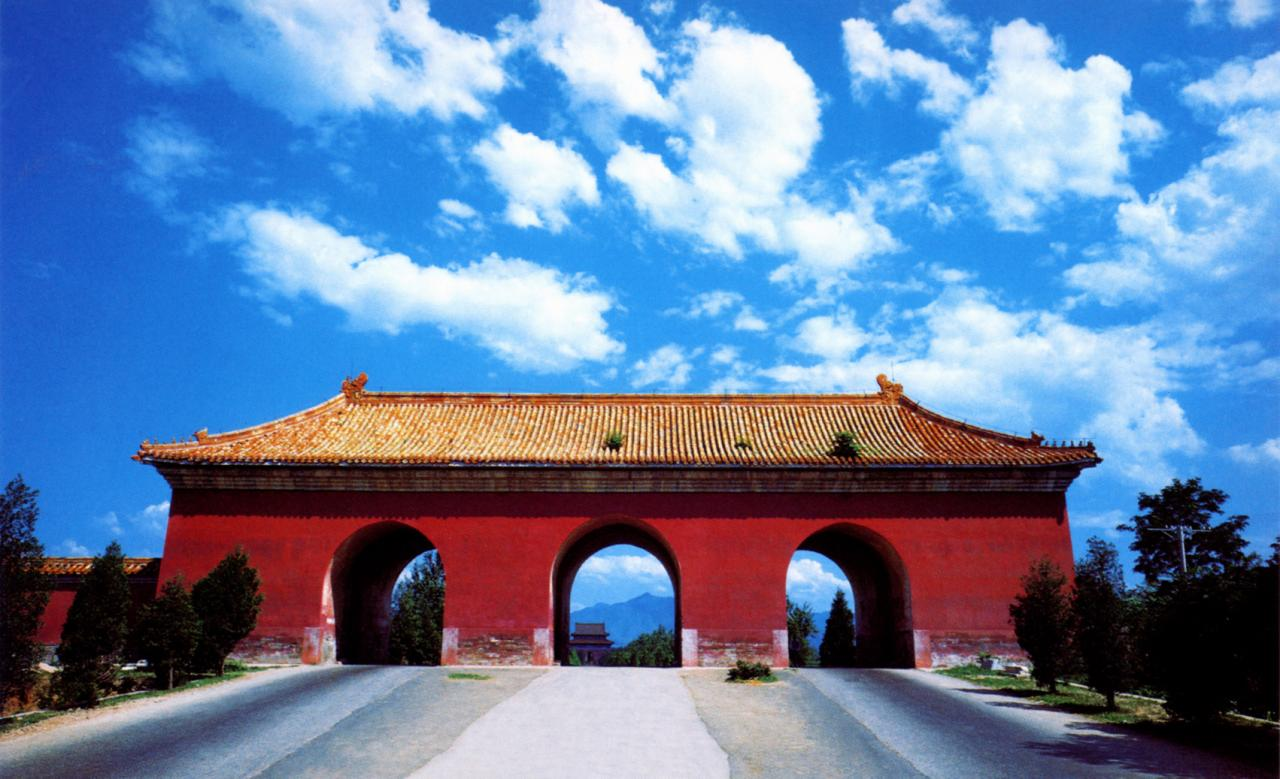
\includegraphics[width=1.0\textwidth]{ShiSan.jpg}
    \end{center}
\end{figure}

\end{document}
